%
% File coling2020.tex
%
% Contact: feiliu@cs.ucf.edu & liang.huang.sh@gmail.com
%% Based on the style files for COLING-2018, which were, in turn,
%% Based on the style files for COLING-2016, which were, in turn,
%% Based on the style files for COLING-2014, which were, in turn,
%% Based on the style files for ACL-2014, which were, in turn,
%% Based on the style files for ACL-2013, which were, in turn,
%% Based on the style files for ACL-2012, which were, in turn,
%% based on the style files for ACL-2011, which were, in turn, 
%% based on the style files for ACL-2010, which were, in turn, 
%% based on the style files for ACL-IJCNLP-2009, which were, in turn,
%% based on the style files for EACL-2009 and IJCNLP-2008...

%% Based on the style files for EACL 2006 by 
%%e.agirre@ehu.es or Sergi.Balari@uab.es
%% and that of ACL 08 by Joakim Nivre and Noah Smith

\documentclass[11pt]{article}
\usepackage{coling2020}
\usepackage{times}
\usepackage{url}
\usepackage{latexsym}
\usepackage{indentfirst}

\usepackage{times}
\usepackage{latexsym}
\usepackage{times}
\usepackage{soul}
\usepackage{url}
\usepackage{amsmath}
\usepackage{amsthm}
\usepackage{booktabs}
\usepackage{algorithm}
\usepackage{algorithmic}
\usepackage{amssymb}
\usepackage{longtable}
\usepackage{graphicx}
\usepackage{CJK}
\usepackage{multirow}
\usepackage{color}
\usepackage{threeparttable}
\usepackage{makecell}
\usepackage{appendix}

\usepackage{algorithm}
\usepackage{algorithmic}
\renewcommand{\algorithmicrequire}{ \textbf{Input:}} %Use Input in the format of Algorithm
\renewcommand{\algorithmicensure}{ \textbf{Output:}} %UseOutput in the format of Algorithm

%\setlength\titlebox{5cm}
\colingfinalcopy % Uncomment this line for the final submission

% You can expand the titlebox if you need extra space
% to show all the authors. Please do not make the titlebox
% smaller than 5cm (the original size); we will check this
% in the camera-ready version and ask you to change it back.

\title{2021年05月05日进度汇报}

\author{屈原斌 \\
首都师范大学 \\
{\tt ybqu@cnu.edu.cn}}

\date{}

\begin{document}
\begin{CJK}{UTF8}{gkai}
\tableofcontents
  
\maketitle
\CJKindent
%\begin{abstract}

%\end{abstract}

\section{今日进度}


\begin{itemize}
  \item [1.] 更新离题检测实验
  \begin{itemize}
    \item \textcolor{red}{补充中文实验,(聚类方案一,表2 / 聚类方案三,表7)}
  \end{itemize}
\end{itemize}

\section{工作详述}
\begin{itemize}
  \item 实验数据(详细信息见附录):
  \begin{itemize}
    \item 英文:ICLE数据集,11个主题,共827篇作文,离题:切题=51:776(1:15)
    \item 中文:智学网初中作文数据,10个主题(35个主题,随机选了10个主题),共5498篇作文,离题:切题=350:5148(1:14.7)
  \end{itemize}
  \item 实验方案:
  \begin{itemize}
    \item 聚类方案一:
    \begin{itemize}
      \item 计算聚类结果中可能离题的类与范文类的相似度,实验结果见表1
      \begin{itemize}
        \item \textcolor{red}{\textbf{调参方式:}}
        \item [-] distance\_threshold:从0-1以0.05步长调参
        \item [-] example\_threshold:大类按照比例调参(对所有类按照作文数排序,当大类包含作文数占比大于阈值时停止)
      \end{itemize} 
      \item linkage取不同参数时指标对比(doc2vec),实验结果见表2
      \item 结论:
      \begin{itemize}
        \item linkage取complete(最大值)时指标最优
        \item [?] bert生成/分类模型,取不同表示时结论不一致
      \end{itemize}
      \item [!] \textcolor{red}{不同表示下spearman相关系数差别较大:}
      \begin{itemize}
        \item 不同表示下相同主题指标最优时小类的作文数不同,会导致一些作文相似度计算方式不同(小类中的作文,取与大类相似度的最小值;大类中作文,取与自己类质心的相似度)
        % \item [?] 大类和小类中的作文混在一起排序
        \item 大类和小类一起排序可能会改变原来的顺序(单独计算大小类的spearman相关系数波动较大)
      \end{itemize}
    \end{itemize}
    \item 聚类方案二(one-class):
    \begin{itemize}
      \item 计算全部作文与它们的质心的相似度,实验结果见表3
      \item 结论:
      \begin{itemize}
        \item bert生成模型指标最优
      \end{itemize}
    \end{itemize}
    \item 聚类方案三(Prompt-independent)
    \begin{itemize}
      \item 五折交叉验证,使用开发集调参,测试集测试,实验结果见表4
      \item 结论:
      \begin{itemize}
        \item 使用开发集的参数测试集测试时,部分主题没有小类(和划分范文类策略相关)
      \end{itemize}
    \end{itemize}
    \item 聚类方案四
    \begin{itemize}
      \item 计算作文与prompt的相似度,进行排序,实验结果见表5
    \end{itemize}
    \item 结论:
    \begin{itemize}
      \item bert生成模型指标最优
    \end{itemize}
  \end{itemize}
\end{itemize}

% 方案一
% Table generated by Excel2LaTeX from sheet '整理(余弦相似度,使用占比划分大小类)'
\begin{table}[hp]\small
  \centering
  \resizebox*{\textwidth}{!}{
    \begin{tabular}{c|c|ccccccccc}
      \hline
      \multicolumn{2}{c|}{} & \textbf{R@10} & \textbf{R@15} & \textbf{R@20} & \textbf{R@50} & \textbf{R@all} & \textbf{P@1} & \textbf{P@5} & \textbf{P@10} & \textbf{spearman} \\
      \hline
      \multicolumn{2}{c|}{\textbf{baseline}} & 0.5334  & 0.5334  & 0.6546  & 0.7548  & 0.8225  & 0.3636  & 0.3091  & 0.2727  & 0.2007  \\
      \hline
      \multicolumn{2}{c|}{\textbf{tfidf}} & 0.5009 & 0.5009 & 0.5517 & 0.6875 & 0.7446 & 0.3636 & 0.2727 & 0.2636 & 0.1866 \\
      \hline
      \multicolumn{2}{c|}{\textbf{doc2vec}} & 0.5334  & 0.6243  & 0.6296  & 0.6888  & 0.7459  & 0.2727  & 0.2727  & 0.2727  & 0.1355  \\
      \hline
      \multirow{7}[0]{*}{\textbf{分类模型}} & \textbf{lstm} & 0.4842  & 0.5023  & 0.5259  & 0.6207  & 0.6635  & 0.4545  & 0.2545  & 0.2364  & 0.1676  \\
      \cline{2-11}
      & \textbf{bert\_CLS} & 0.5995  & 0.5995  & 0.6298  & 0.7064  & 0.7545  & 0.2727  & 0.2727  & 0.2727  & 0.1776  \\
      & \textbf{bert\_CLS}(+whitening) & 0.6093  & 0.6449  & 0.6449  & 0.7055  & 0.8000  & 0.1818  & 0.2727  & 0.2636  & 0.1426  \\
      \cline{2-11}
      & \textbf{bert\_Last1avg} & 0.5540  & 0.6752  & 0.7358  & 0.7465  & 0.7947  & 0.3636  & 0.2727  & 0.2818  & 0.1977  \\
      & \textbf{bert\_Last1avg}(+whitening) & 0.7002  & 0.7358  & 0.7412  & 0.7768  & 0.8303  & 0.3636  & 0.2909  & 0.3000  & 0.2111  \\
      \cline{2-11}
      & \textbf{bert\_Last2avg} & 0.5540  & 0.6752  & 0.6752  & 0.7647  & 0.8128  & 0.2727  & 0.2909  & 0.2818  & 0.1745  \\
      & \textbf{bert\_Last2avg}(+whitening) & 0.5357  & 0.5357  & 0.6266  & 0.6911  & 0.7392  & 0.1818  & 0.2727  & 0.2636  & 0.1551  \\
      \hline
      \multirow{12}[0]{*}{\textbf{生成模型}} & \textbf{lstm\_$\rm h_{t_n}$} & 0.3781  & 0.3834  & 0.3834  & 0.4979  & 0.5460  & 0.0909  & 0.1636  & 0.2000  & 0.0792  \\
      & \textbf{lstm\_avg} & 0.4394  & 0.4697  & 0.4697  & 0.6016  & 0.6658  & 0.2727  & 0.2182  & 0.2182  & 0.1148  \\
      & \textbf{lstm\_$\rm h_{t_n}$}(+作文) & 0.4189  & 0.4319  & 0.4319  & 0.6191  & 0.6191  & 0.0000  & 0.1273  & 0.2182  & 0.0009  \\
      & \textbf{lstm\_avg}(+作文) & 0.4582  & 0.4635  & 0.4635  & 0.4999  & 0.4999  & 0.0909  & 0.1455  & 0.1818  & 0.0264  \\
      \cline{2-11}
      & \textbf{bert\_CLS} & 0.4526  & 0.4579  & 0.4579  & 0.4579  & 0.4579  & 0.1818  & 0.2000  & 0.1818  & 0.1146  \\
      & \textbf{bert\_CLS}(+whitening) & 0.5963  & 0.5963  & 0.6319  & 0.7531  & 0.8066  & 0.3636  & 0.2545  & 0.2727  & 0.1594  \\
      & \textbf{bert\_CLS}(+作文) & 0.4944  & 0.4998  & 0.4998  & 0.5105  & 0.5319  & 0.3636  & 0.2545  & 0.2364  & 0.0420  \\
      & \textbf{bert\_CLS}(+作文,+wihtening) & 0.6038  & 0.6038  & 0.6038  & 0.7592  & 0.7753  & 0.0909  & 0.2545  & 0.2818  & 0.0800  \\
      \cline{2-11}
      & \textbf{bert\_Last1avg} & 0.5500  & 0.6409  & 0.6560  & 0.6863  & 0.6863  & 0.4545  & 0.2545  & 0.2545  & 0.1250  \\
      & \textbf{bert\_Last1avg}(+whitening) & \textcolor[rgb]{ 1,  0,  0}{\textbf{0.7023 }} & 0.7023  & 0.7023  & 0.7433  & 0.7487  & 0.2727  & 0.2727  & 0.2909  & 0.1523  \\
      & \textbf{bert\_Last1avg}(+作文) & 0.4739  & 0.4793  & 0.4793  & 0.5256  & 0.5310  & 0.4545  & 0.2727  & 0.2273  & 0.0324  \\
      & \textbf{bert\_Last1avg}(+作文,+whitening) & 0.6925  & 0.6925  & 0.7228  & 0.7517  & 0.7892  & 0.3636  & 0.3091  & 0.3000  & 0.2039  \\
      \hline
    \end{tabular}%
  }
  \begin{tablenotes}    %这行要添加, 从这开始
    \footnotesize               %这行要添加
    \item[1] R@all 表示全部小类中离题的召回
    \item[2] +作文 表示在作文数据上进行微调(原始模型使用新闻数据预训练) 
    \item[3] +whitening 表示使用Bert-whitening对表示进行变换
    \item[4] * lstm\_$\rm h_{t_n}$ 表示取Lstm最后时刻的表示,lstm\_avg 表示取Lstm所有时刻的表示平均 
  \end{tablenotes} 
  \caption{聚类方案一指标更新(英文)}
  \label{tab:addlabel}%
\end{table}%

% Table generated by Excel2LaTeX from sheet '中文整理(10主题)'
\begin{table}[htbp]
  \centering
  \resizebox*{\textwidth}{!}{
    \begin{tabular}{c|c|ccccccccc}
      \hline
      \multicolumn{2}{c|}{} & \textbf{R@10} & \textbf{R@15} & \textbf{R@20} & \textbf{R@50} & \textbf{R@all} & \textbf{P@1} & \textbf{P@5} & \textbf{P@10} & \textbf{spearman} \\
      \hline
      \multicolumn{2}{c|}{\textbf{tfidf}} &       &       &       &       &       &       &       &       &  \\
      \hline
      \multicolumn{2}{c|}{\textbf{doc2vec}} & 0.2185  & 0.3183  & 0.3902  & 0.8091  & 0.9190  & 0.8000  & 0.8000  & 0.7500  & 0.6813  \\
      \hline
      \multirow{10}[0]{*}{\textbf{分类模型}} & \textbf{lstm} & 0.2054  & 0.2975  & 0.3949  & 0.8509  & 0.9632  & 0.6000  & 0.7200  & 0.7000  & 0.7036  \\
      & \textbf{lstm(+测试主题)} & 0.2078  & 0.3052  & 0.4010  & 0.8346  & 0.9225  & 0.8000  & 0.7600  & 0.7200  & 0.6853  \\
      \cline{2-11}
      & \textbf{bert\_CLS} & 0.2056  & 0.2882  & 0.3851  & 0.7911  & 0.8706  & 0.6000  & 0.6800  & 0.7000  & 0.6574  \\
      & \textbf{bert\_CLS(+whitening)} & 0.2101  & 0.3057  & 0.4126  & 0.7884  & 0.8762  & 0.7000  & 0.7600  & 0.7200  & 0.6489  \\
      & \textbf{bert\_CLS(+测试主题)} & 0.2076  & 0.3066  & 0.4079  & 0.8208  & 0.9192  & 0.6000  & 0.6600  & 0.7100  & 0.6384  \\
      & \textbf{bert\_CLS(+测试主题,+whitening)} & 0.2015  & 0.3035  & 0.3929  & 0.8009  & 0.8894  & 0.8000  & 0.6400  & 0.7000  & 0.6670  \\
      \cline{2-11}
      & \textbf{bert\_Last1avg} & 0.2053  & 0.3038  & 0.3886  & 0.7581  & 0.8610  & 0.7000  & 0.6600  & 0.7000  & 0.6629  \\
      & \textbf{bert\_Last1avg(+whitening)} & 0.2131  & 0.2928  & 0.3767  & 0.7686  & 0.8836  & 0.6000  & 0.7400  & 0.7300  & 0.6238  \\
      & \textbf{bert\_Last1avg(+测试主题)} & 0.2158  & 0.3199  & 0.4128  & 0.8339  & 0.9565  & 0.9000  & 0.8200  & 0.7300  & 0.7060  \\
      & \textbf{bert\_Last1avg(+测试主题,+whitening)} & 0.2112  & 0.3184  & 0.4251  & 0.8291  & 0.9319  & 0.8000  & 0.7000  & 0.7300  & 0.6638  \\
      \hline
      \multirow{10}[0]{*}{\textbf{生成模型}} & \textbf{lstm\_$\rm h_{t_n}$} & 0.1534  & 0.2230  & 0.3174  & 0.7315  & 0.8548  & 0.5000  & 0.4000  & 0.5500  & 0.6310  \\
      & \textbf{lstm\_avg} & 0.2063  & 0.2900  & 0.3893  & 0.7935  & 0.9107  & 0.7000  & 0.6800  & 0.7200  & 0.7018  \\
      \cline{2-11}
      & \textbf{bert\_CLS} & 0.1896  & 0.2744  & 0.3540  & 0.7248  & 0.8743  & 0.8000  & 0.7000  & 0.6600  & 0.6063  \\
      & \textbf{bert\_CLS(+whitening)} & 0.2247  & 0.2947  & 0.3888  & 0.7240  & 0.8910  & 0.7000  & 0.7400  & 0.7700  & 0.6184  \\
      & \textbf{bert\_CLS(+测试作文)} & 0.0351  & 0.0523  & 0.0724  & 0.1276  & 0.1866  & 0.3000  & 0.1400  & 0.1300  & 0.0361  \\
      & \textbf{bert\_CLS(+测试作文,+wihtening)} & \textbf{\textcolor{red}{0.2293}}  & 0.3020  & 0.3755  & 0.7813  & 0.9065  & 0.9000  & 0.8400  & 0.7800  & 0.6702  \\
      \cline{2-11}
      & \textbf{bert\_Last1avg} & 0.1674  & 0.2369  & 0.3258  & 0.6856  & 0.8351  & 0.7000  & 0.6200  & 0.5800  & 0.5955  \\
      & \textbf{bert\_Last1avg(+whitening)} & 0.2086  & 0.2754  & 0.3496  & 0.6395  & 0.7704  & 0.8000  & 0.6600  & 0.7200  & 0.5511  \\
      & \textbf{bert\_Last1avg(+测试作文)} & 0.0543  & 0.0716  & 0.0791  & 0.1349  & 0.2437  & 0.5000  & 0.2800  & 0.2100  & 0.0522  \\
      & \textbf{bert\_Last1avg(+测试作文,+whitening)} & 0.2171  & 0.3102  & 0.3822  & 0.7524  & 0.8923  & 0.8000  & 0.8000  & 0.7500  & 0.6608  \\
      \hline
    \end{tabular}}%
    \begin{tablenotes}    %这行要添加, 从这开始
      \footnotesize               %这行要添加
      % \item[1] R@all 表示全部小类中离题的召回
      \item[2] +测试主题 表示在测试主题继续训练分类模型;+测试作文 表示在测试集上继续训练生成模型
      % \item[4] +whitening 表示使用Bert-whitening对表示进行变换
      \item[5] * lstm\_$\rm h_{t_n}$ 表示取Lstm最后时刻的表示,lstm\_avg 表示取Lstm所有时刻的表示平均 
    \end{tablenotes} 
    \caption{聚类方案一指标更新(中文)}
  \label{tab:addlabel}%
\end{table}%


% Table generated by Excel2LaTeX from sheet '整理(余弦相似度,使用占比划分大小类)'
\begin{table}[hp]\small
  \centering
    \begin{tabular}{c|ccccccccc}
      \hline
      \textcolor[rgb]{ 1,  0,  0}{} & \multicolumn{1}{c}{\textbf{R@10}} & \multicolumn{1}{c}{\textbf{R@15}} & \multicolumn{1}{c}{\textbf{R@20}} & \multicolumn{1}{c}{\textbf{R@50}} & \multicolumn{1}{c}{\textbf{R@all}} & \multicolumn{1}{c}{\textbf{P@1}} & \multicolumn{1}{c}{\textbf{P@5}} & \multicolumn{1}{c}{\textbf{P@10}} & \multicolumn{1}{c}{\textbf{spearman}} \\
      \hline
      \textbf{linkage='average'} & 0.5334  & 0.6243  & 0.6296  & 0.6888  & 0.7459  & 0.2727  & 0.2727  & 0.2727  & 0.1355  \\
      \hline
      \textbf{linkage='complete'} & \textcolor[rgb]{ 1,  0,  0}{\textbf{0.6849 }} & 0.6849  & 0.6902  & 0.7312  & 0.7883  & 0.2727  & 0.3091  & 0.3000  & 0.1504  \\
      \hline
      \textbf{linkage='single'} & 0.5001  & 0.6061  & 0.6061  & 0.6781  & 0.7459  & 0.4545  & 0.2727  & 0.2545  & 0.1573  \\
      \hline
    \end{tabular}%
    \begin{tablenotes}
      \item[1] linkage='average': 取平均;linkage='complete': 取最大值;linkage='single': 取最小值;
    \end{tablenotes}
    \caption{linkage取不同参数时指标对比(英文,doc2vec)}
  \label{tab:addlabel}%
\end{table}%

% 方案二
% Table generated by Excel2LaTeX from sheet '整理(余弦相似度,使用占比划分大小类)'
\begin{table}[hp]
  \centering
  \resizebox*{\textwidth}{!}{
    \begin{tabular}{c|c|ccccccccc}
      \hline
      \multicolumn{2}{c|}{} & \textbf{R@10} & \textbf{R@15} & \textbf{R@20} & \textbf{R@50} & \textbf{R@all} & \textbf{P@1} & \textbf{P@5} & \textbf{P@10} & \textbf{spearman} \\
      \hline
      \multicolumn{2}{c|}{\textbf{baseline}} & 0.3917  & 0.4631  & 0.5594  & 0.7148  & -     & 0.4545  & 0.2909  & 0.2182  & 0.1429  \\
      \hline
      \multicolumn{2}{c|}{\textbf{tfidf}} & 0.4350  & 0.4533  & 0.5041  & 0.7558  & -     & 0.4545  & 0.3091  & 0.2364  & 0.2437  \\
      \hline
      \multicolumn{2}{c|}{\textbf{doc2vec}} & 0.3865  & 0.4381  & 0.5291  & 0.7041  & -     & 0.5455  & 0.2727  & 0.2182  & 0.1865  \\
      \hline
      \multirow{7}[0]{*}{\textbf{分类模型}} & \textbf{lstm} & 0.3728  & 0.4062  & 0.4479  & 0.7398  & -     & 0.4545  & 0.2727  & 0.1909  & 0.1535  \\
      \cline{2-11}
      & \textbf{bert\_CLS} & 0.3029  & 0.4480  & 0.5419  & 0.7344  & -     & 0.2727  & 0.2182  & 0.1818  & 0.0960  \\
      & \textbf{bert\_CLS(+whitening)} & 0.2977  & 0.3918  & 0.4578  & 0.7398  & -     & 0.2727  & 0.1636  & 0.1636  & 0.1833  \\
      \cline{2-11}
      & \textbf{bert\_Last1avg} & 0.3635  & 0.4480  & 0.4934  & 0.7291  & -     & 0.3636  & 0.2364  & 0.2000  & 0.1101  \\
      & \textbf{bert\_Last1avg(+whitening)} & 0.3637  & 0.4221  & 0.4631  & 0.7451  & -     & 0.3636  & 0.2364  & 0.2000  & 0.2126  \\
      \cline{2-11}
      & \textbf{bert\_Last2avg} & 0.3582  & 0.4176  & 0.4631  & 0.7291  & -     & 0.2727  & 0.2545  & 0.1909  & 0.1189  \\
      & \textbf{bert\_Last2avg(+whitening)} & 0.3084  & 0.3873  & 0.4381  & 0.6381  & -     & 0.2727  & 0.2364  & 0.1909  & 0.1725  \\
      \hline
      \multirow{12}[0]{*}{\textbf{生成模型}} & \textbf{lstm\_$\rm h_{t_n}$} & 0.1826  & 0.2850  & 0.4062  & 0.6684  & -     & 0.0909  & 0.1273  & 0.1091  & 0.0156  \\
      & \textbf{lstm\_avg} & 0.3455  & 0.3736  & 0.4070  & 0.6025  & -     & 0.1818  & 0.1636  & 0.1818  & 0.0765  \\
      & \textbf{lstm\_$\rm h_{t_n}$(+作文)} & 0.1263  & 0.2463  & 0.3676  & 0.7041  & -     & 0.0000  & 0.0727  & 0.0818  & -0.0039  \\
      & \textbf{lstm\_avg(+作文)} & 0.1792  & 0.3394  & 0.4788  & 0.7023  & -     & 0.0909  & 0.1273  & 0.1000  & -0.0041  \\
      \cline{2-11}
      & \textbf{bert\_CLS} & 0.3476  & 0.6214  & 0.6820  & 0.8503  & -     & 0.1818  & 0.2182  & 0.1818  & 0.1516  \\
      & \textbf{bert\_CLS(+whitening)} & 0.4371  & 0.4813  & 0.5570  & 0.7344  & -     & 0.2727  & 0.2909  & 0.2091  & 0.1300  \\
      & \textbf{bert\_CLS(+作文)} & \textcolor[rgb]{ 1,  0,  0}{\textbf{0.5259 }} & 0.5389  & 0.5389  & 0.7504  & -     & 0.3636  & 0.2364  & 0.2636  & 0.1266  \\
      & \textbf{bert\_CLS(+作文,+wihtening)} & 0.3810  & 0.4373  & 0.5184  & 0.6988  & -     & 0.2727  & 0.2727  & 0.1909  & 0.1038  \\
      \cline{2-11}
      & \textbf{bert\_Last1avg} & 0.3393  & 0.5328  & 0.6873  & 0.8449  & -     & 0.4545  & 0.2182  & 0.1727  & 0.1026  \\
      & \textbf{bert\_Last1avg(+whitening)} & 0.3152  & 0.4547  & 0.5335  & 0.7594  & -     & 0.2727  & 0.2182  & 0.1727  & 0.1071  \\
      & \textbf{bert\_Last1avg(+作文)} & 0.5107  & 0.5389  & 0.5389  & 0.7451  & -     & 0.3636  & 0.2909  & 0.2545  & 0.1280  \\
      & \textbf{bert\_Last1avg(+作文,+whitening)} & 0.3658  & 0.4827  & 0.5736  & 0.8004  & -     & 0.2727  & 0.2000  & 0.1909  & 0.1177  \\
      \hline
    \end{tabular}%
  }
  \begin{tablenotes}    %这行要添加, 从这开始
    \footnotesize               %这行要添加
    \item[1] R@all 表示全部小类中离题的召回
    \item[2] +作文 表示在作文数据上进行微调(原始模型使用新闻数据预训练) 
    \item[2] +whitening 表示使用Bert-whitening对表示进行变换
    \item[3] * lstm\_$\rm h_{t_n}$ 表示取Lstm最后时刻的表示,lstm\_avg 表示取Lstm所有时刻 
  \end{tablenotes} 
  \caption{聚类方案二(one-class)指标更新(英文)}
  \label{tab:addlabel}%
\end{table}%

% Table generated by Excel2LaTeX from sheet '中文整理(10主题)'
\begin{table}[htbp]
  \centering
  \resizebox*{\textwidth}{!}{
    \begin{tabular}{c|c|ccccccccc}
      \hline
      \multicolumn{2}{c|}{} & \textbf{R@10} & \textbf{R@15} & \textbf{R@20} & \textbf{R@50} & \textbf{R@all} & \textbf{P@1} & \textbf{P@5} & \textbf{P@10} & \textbf{spearman} \\
      \hline
      \multicolumn{2}{c|}{\textbf{tfidf}} & 0.0621  & 0.0956  & 0.1138  & 0.2151  & -     & 0.2000  & 0.2400  & 0.2300  & 0.0956  \\
      \hline
      \multicolumn{2}{c|}{\textbf{doc2vec}} & 0.0428  & 0.0594  & 0.0962  & 0.2191  & -     & 0.2000  & 0.1400  & 0.1600  & 0.1057  \\
      \hline
      \multirow{10}[0]{*}{\textbf{分类模型}} & \textbf{lstm} & 0.0615  & 0.0905  & 0.1072  & 0.2314  & -     & 0.4000  & 0.2600  & 0.2300  & 0.1343  \\
      & \textbf{lstm(+测试主题)} & \textcolor[rgb]{ 1,  0,  0}{\textbf{0.1038 }} & 0.1479  & 0.1781  & 0.3175  & -     & 0.5000  & 0.4600  & 0.3700  & 0.1616  \\
      \cline{2-11}
      & \textbf{bert\_CLS} & 0.0624  & 0.0894  & 0.1006  & 0.2223  & -     & 0.6000  & 0.2400  & 0.2200  & 0.1106  \\
      & \textbf{bert\_CLS(+whitening)} & 0.0236  & 0,0415 & 0,0605 & 0.1893  & -     & 0.1000  & 0,1000 & 0.0900  & 0,0995 \\
      & \textbf{bert\_CLS(+测试主题)} & 0.0677  & 0.0837  & 0.1136  & 0.2448  & -     & 0.2000  & 0.3200  & 0.2500  & 0.1454  \\
      & \textbf{bert\_CLS(+测试主题,+whitening)} & 0.0619  & 0.0744  & 0.1000  & 0.2204  & -     & 0.4000  & 0.2600  & 0.2300  & 0.1266  \\
      \cline{2-11}
      & \textbf{bert\_Last1avg} & 0.0611  & 0.0811  & 0.1022  & 0.2172  & -     & 0.3000  & 0.2400  & 0.2100  & 0.0991  \\
      & \textbf{bert\_Last1avg(+whitening)} & 0.0622  & 0.0834  & 0.1033  & 0.2103  & -     & 0.4000  & 0.2800  & 0.2300  & 0.1060  \\
      & \textbf{bert\_Last1avg(+测试主题)} & 0.0853  & 0.1217  & 0.1462  & 0.2877  & -     & 0.5000  & 0.3200  & 0.2900  & 0.1725  \\
      & \textbf{bert\_Last1avg(+测试主题,+whitening)} & 0.0796  & 0.1097  & 0.1378  & 0.3037  & -     & 0.5000  & 0.3000  & 0.2900  & 0.1650  \\
      \hline
      \multirow{10}[0]{*}{\textbf{生成模型}} & \textbf{lstm\_$\rm h_{t_n}$} & 0.0129  & 0.0241  & 0.0292  & 0.1073  & -     & 0.0000  & 0.0600  & 0.0500  & 0.0086  \\
      & \textbf{lstm\_avg} & 0.0526  & 0.0751  & 0.0930  & 0.1964  & -     & 0.3000  & 0.2400  & 0.1900  & 0.0977  \\
      \cline{2-11}
      & \textbf{bert\_CLS} & 0.0669  & 0.0878  & 0.1111  & 0.2064  & -     & 0.3000  & 0.3000  & 0.2500  & 0.0624  \\
      & \textbf{bert\_CLS(+whitening)} & 0.0793  & 0.0987  & 0.1162  & 0.2312  & -     & 0.5000  & 0.4000  & 0.2900  & 0.0848  \\
      & \textbf{bert\_CLS(+测试作文)} & 0.0337  & 0.0472  & 0.0639  & 0.1519  & -     & 0.1000  & 0.1600  & 0.1300  & 0.0162  \\
      & \textbf{bert\_CLS(+测试作文,+wihtening)} & 0.0630  & 0.0841  & 0.0957  & 0.2028  & -     & 0.3000  & 0.2600  & 0.2300  & 0.0624  \\
      \cline{2-11}
      & \textbf{bert\_Last1avg} & 0.0566  & 0.0721  & 0.0787  & 0.1745  & -     & 0.1000  & 0.2000  & 0.2000  & 0.0564  \\
      & \textbf{bert\_Last1avg(+whitening)} & 0.0593  & 0.0842  & 0.1106  & 0.2061  & -     & 0.3000  & 0.2200  & 0.2200  & 0.0828  \\
      & \textbf{bert\_Last1avg(+测试作文)} & 0.0495  & 0.0628  & 0,0726 & 0.1507  & -     & 0.5000  & 0.2800  & 0.1900  & 0.0280  \\
      & \textbf{bert\_Last1avg(+测试作文,+whitening)} & 0.0669  & 0.0878  & 0.1037  & 0.2074  & -     & 0.1000  & 0.2000  & 0.2400  & 0.0646  \\
      \hline
    \end{tabular}}%
    \begin{tablenotes}    %这行要添加, 从这开始
      \footnotesize               %这行要添加
      % \item[1] R@all 表示全部小类中离题的召回
      \item[2] +测试主题 表示在测试主题继续训练分类模型; +测试作文 表示在测试集上继续训练生成模型
      % \item[4] +whitening 表示使用Bert-whitening对表示进行变换
      \item[5] * lstm\_$\rm h_{t_n}$ 表示取Lstm最后时刻的表示,lstm\_avg 表示取Lstm所有时刻的表示平均 
    \end{tablenotes} 
    \caption{聚类方案二(one-class)指标更新(中文)}
  \label{tab:addlabel}%
\end{table}%

% 方案三
% Table generated by Excel2LaTeX from sheet '整理(余弦相似度,使用占比划分大小类)'
\begin{table}[hp]\small
  \centering
  \resizebox*{\textwidth}{!}{
    \begin{tabular}{c|c|ccccccccc}
      \hline
      \multicolumn{2}{c|}{} & \textbf{R@10} & \textbf{R@15} & \textbf{R@20} & \textbf{R@50} & \textbf{R@all} & \textbf{P@1} & \textbf{P@5} & \textbf{P@10} & \textbf{spearman} \\
      \hline
      \multicolumn{2}{c|}{\textbf{baseline}} & 0.1070  & 0.1070  & 0.1123  & 0.3351  & 0.3779  & 0.0000  & 0.0909  & 0.0545  & 0.0197  \\
      \hline
      \multicolumn{2}{c|}{\textbf{tfidf}} & 0.0667 & 0.0667 & 0.0970 & 0.1758 & 0.1758 & 0.0909 & 0.0545 & 0.0273 & 0.0233 \\
      \hline
      \multicolumn{2}{c|}{\textbf{doc2vec}} & 0.1468  & 0.2256  & 0.2256  & 0.5129  & 0.5343  & 0.0909  & 0.1273  & 0.0909  & 0.1160  \\
      \hline
      \multirow{7}[0]{*}{\textbf{分类模型}} & \textbf{lstm} & 0.0645  & 0.1184  & 0.1668  & 0.2791  & 0.3219  & 0.0909  & 0.0182  & 0.0455  & 0.0089  \\
      \cline{2-11}
      & \textbf{bert\_CLS} & 0.2371  & 0.2674  & 0.3280  & 0.5259  & 0.5580  & 0.1818  & 0.1636  & 0.1455  & 0.1018  \\
      & \textbf{bert\_CLS(+whitening)} & 0.2576  & 0.2986  & 0.2986  & 0.5517  & 0.5892  & 0.0909  & 0.1636  & 0.1455  & 0.0950  \\
      \cline{2-11}
      & \textbf{bert\_Last1avg} & 0.1982  & 0.2285  & 0.2891  & 0.5119  & 0.5386  & 0.2727  & 0.1636  & 0.1182  & 0.0908  \\
      & \textbf{bert\_Last1avg(+whitening)} & 0.2145  & 0.3539  & 0.3895  & 0.5517  & 0.5785  & 0.1818  & 0.1636  & 0.1364  & 0.0739  \\
      \cline{2-11}
      & \textbf{bert\_Last2avg} & 0.2231  & 0.2891  & 0.3194  & 0.5172  & 0.5333  & 0.1818  & 0.1636  & 0.1182  & 0.0960  \\
      & \textbf{bert\_Last2avg(+whitening)} & 0.1527  & 0.1527  & 0.1830  & 0.3256  & 0.3577  & 0.0909  & 0.1455  & 0.0909  & 0.0329  \\
      \hline
      \multirow{11}[0]{*}{\textbf{生成模型}} & \textbf{lstm\_$\rm h_{t_n}$} & 0.1273  & 0.2182  & 0.2182  & 0.2699  & 0.2752  & 0.0909  & 0.0545  & 0.0636  & 0.0045  \\
      & \textbf{lstm\_avg} & 0.1857  & 0.2062  & 0.2365  & 0.3631  & 0.3952  & 0.0000  & 0.1273  & 0.1000  & 0.0418  \\
      & \textbf{lstm\_$\rm h_{t_n}$(+作文)} & 0.0766  & 0.1426  & 0.1715  & 0.2231  & 0.2392  & 0.0000  & 0.0545  & 0.0455  & 0.0009  \\
      & \textbf{lstm\_avg(+作文)} & 0.1447  & 0.1750  & 0.2053  & 0.2517  & 0.2731  & 0.0909  & 0.0909  & 0.0727  & -0.0207  \\
      \cline{2-11}
      & \textbf{bert\_CLS} & 0.3501  & 0.3554  & 0.3661  & 0.3715  & 0.3715  & 0.1818  & 0.1636  & 0.1182  & 0.1271  \\
      & \textbf{bert\_CLS(+whitening)} & 0.2452  & 0.3195  & 0.3801  & 0.5174  & 0.6511  & 0.2727  & 0.1636  & 0.1273  & 0.0635  \\
      & \textbf{bert\_CLS(+作文)} & 0.3873  & 0.4480  & 0.4533  & 0.4943  & 0.5103  & 0.2727  & 0.2545  & 0.1909  & 0.0662  \\
      & \textbf{bert\_CLS(+作文,+wihtening)} & \textbf{\textcolor{red}{0.3885}}  & 0.4143  & 0.4143  & 0.5894  & 0.7070  & 0.3636  & 0.2364  & 0.2000  & 0.0692  \\
      \cline{2-11}
      & \textbf{bert\_Last1avg} & 0.2549  & 0.3390  & 0.4602  & 0.6224  & 0.6331  & 0.2727  & 0.2182  & 0.1273  & 0.0413  \\
      & \textbf{bert\_Last1avg(+whitening)} & 0.1937  & 0.3937  & 0.4421  & 0.5067  & 0.5281  & 0.2727  & 0.1273  & 0.1091  & 0.0036  \\
      & \textbf{bert\_Last1avg(+作文)} & 0.3009  & 0.3062  & 0.3971  & 0.4078  & 0.4078  & 0.3636  & 0.2000  & 0.1455  & 0.0407  \\
      & \textbf{bert\_Last1avg(+作文,+whitening)} & 0.3097  & 0.3454  & 0.4090  & 0.6803  & 0.7177  & 0.3636  & 0.2364  & 0.1727  & 0.0426  \\
      \hline
    \end{tabular}%
    }
    \begin{tablenotes}    %这行要添加, 从这开始
      \footnotesize               %这行要添加
      \item[1] R@all 表示全部小类中离题的召回
      \item[2] +作文 表示在作文数据上进行微调(原始模型使用新闻数据预训练) 
      \item[3] +whitening 表示使用Bert-whitening对表示进行变换
      \item[4] * lstm\_$\rm h_{t_n}$ 表示取Lstm最后时刻的表示,lstm\_avg 表示取Lstm所有时刻的表示平均
    \end{tablenotes} 
    \caption{聚类方案三(prompt-independent)指标更新(英文)}
  \label{tab:addlabel}%
\end{table}%

% Table generated by Excel2LaTeX from sheet '中文整理(10主题)'
\begin{table}[htbp]
  \centering
  \resizebox*{\textwidth}{!}{
    \begin{tabular}{c|c|ccccccccc}
      \hline
      \multicolumn{2}{c|}{} & \textbf{R@10} & \textbf{R@15} & \textbf{R@20} & \textbf{R@50} & \textbf{R@all} & \textbf{P@1} & \textbf{P@5} & \textbf{P@10} & \textbf{spearman} \\
      \hline
      \multicolumn{2}{c|}{\textbf{tfidf}} &       &       &       &       &       &       &       &       &  \\
      \hline
      \multicolumn{2}{c|}{\textbf{doc2vec}} & 0.1369  & 0.1993  & 0.2476  & 0.5299  & 0.6344  & 0.6000  & 0.6000  & 0.5100  & 0.4823  \\
      \hline
      \multirow{10}[0]{*}{\textbf{分类模型}} & \textbf{lstm} & 0.1313  & 0.1989  & 0.2483  & 0.5323  & 0.6215  & 0.4000  & 0.4800  & 0.4800  & 0.4328  \\
      & \textbf{lstm(+测试主题)} & 0.1207  & 0.1857  & 0.2368  & 0.4925  & 0.5869  & 0.5000  & 0.5000  & 0.4400  & 0.3906  \\
      \cline{2-11}
      & \textbf{bert\_CLS} & 0.1090  & 0.1710  & 0.2120  & 0.4438  & 0.5102  & 0.3000  & 0.3800  & 0.3900  & 0.3225  \\
      & \textbf{bert\_CLS(+whitening)} & 0.1222  & 0.1852  & 0.2471  & 0.4572  & 0.5403  & 0.4000  & 0.4000  & 0.4100  & 0.3688  \\
      & \textbf{bert\_CLS(+测试主题)} & \textbf{\textcolor{red}{0.1692}}  & 0.2562  & 0.3397  & 0.6465  & 0.7374  & 0.6000  & 0.5800  & 0.6100  & 0.4346  \\
      & \textbf{bert\_CLS(+测试主题,+whitening)} & \textbf{\textcolor{green}{0.1018}}  & 0.1599  & 0.2006  & 0.4021  & 0.4399  & 0.3000  & 0.3600  & 0.3700  & 0.3352  \\
      \cline{2-11}
      & \textbf{bert\_Last1avg} & 0.1081  & 0.1576  & 0.2123  & 0.3992  & 0.4927  & 0.4000  & 0.4200  & 0.4000  & 0.3294  \\
      & \textbf{bert\_Last1avg(+whitening)} & 0.1163  & 0.1555  & 0.1970  & 0.3705  & 0.4708  & 0.3000  & 0.3800  & 0.4000  & 0.3549  \\
      & \textbf{bert\_Last1avg(+测试主题)} & 0.1183  & 0.1794  & 0.2473  & 0.4719  & 0.5218  & 0.6000  & 0.5000  & 0.4400  & 0.3568  \\
      & \textbf{bert\_Last1avg(+测试主题,+whitening)} & 0.1268  & 0.2022  & 0.2583  & 0.4808  & 0.5861  & 0.5000  & 0.4400  & 0.4600  & 0.4497  \\
      \hline
      \multirow{10}[0]{*}{\textbf{生成模型}} & \textbf{lstm\_$\rm h_{t_n}$} & 0.0962  & 0.1452  & 0.2001  & 0.4682  & 0.5370  & 0.4000  & 0.3200  & 0.3700  & 0.3994  \\
      & \textbf{lstm\_avg} & 0.1293  & 0.1738  & 0.2275  & 0.4096  & 0.5114  & 0.5000  & 0.4600  & 0.4400  & 0.3856  \\
      \cline{2-11}
      & \textbf{bert\_CLS} & 0.1313  & 0.1989  & 0.2483  & 0.5323  & 0.6215  & 0.4000  & 0.4800  & 0.4800  & 0.4328  \\
      & \textbf{bert\_CLS(+whitening)} & 0.0916  & 0.1359  & 0.1650  & 0.3313  & 0.5222  & 0.4000  & 0.3600  & 0.3100  & 0.3120  \\
      & \textbf{bert\_CLS(+测试作文)} & 0.0327  & 0.0475  & 0.0621  & 0.1054  & 0.1244  & 0.2000  & 0.1400  & 0.1200  & 0.0248  \\
      & \textbf{bert\_CLS(+测试作文,+wihtening)} & 0.0856  & 0.1206  & 0.1505  & 0.2957  & 0.4135  & 0.2000  & 0.3400  & 0.3200  & 0.3255  \\
      \cline{2-11}
      & \textbf{bert\_Last1avg} & 0.1333  & 0.1812  & 0.2581  & 0.6099  & 0.7734  & 0.6000  & 0.5400  & 0.4600  & 0.5095  \\
      & \textbf{bert\_Last1avg(+whitening)} & 0.1648  & 0.2476  & 0.3332  & 0.6212  & 0.7521  & 0.7000  & 0.5800  & 0.5700  & 0.6053  \\
      & \textbf{bert\_Last1avg(+测试作文)} & 0.0519  & 0.0665  & 0.0857  & 0.1460  & 0.1901  & 0.5000  & 0.2800  & 0.2000  & 0.0378  \\
      & \textbf{bert\_Last1avg(+测试作文,+whitening)} & 0.0825  & 0.1226  & 0.1539  & 0.3038  & 0.4135  & 0.4000  & 0.3400  & 0.3100  & 0.3210  \\
      \hline
    \end{tabular}}%
    \begin{tablenotes}    %这行要添加, 从这开始
      \footnotesize               %这行要添加
      % \item[1] R@all 表示全部小类中离题的召回
      \item[2] +测试主题 表示在测试主题继续训练分类模型;+测试作文 表示在测试集上继续训练生成模型
      % \item[4] +whitening 表示使用Bert-whitening对表示进行变换
      \item[5] * lstm\_$\rm h_{t_n}$ 表示取Lstm最后时刻的表示,lstm\_avg 表示取Lstm所有时刻的表示平均 
    \end{tablenotes} 
    \caption{聚类方案三(prompt-independent)指标更新(中文)}
  \label{tab:addlabel}%
\end{table}%


% 方案四
% Table generated by Excel2LaTeX from sheet '整理(余弦相似度,使用占比划分大小类)'
\begin{table}[htbp]\small
  \centering
  \resizebox*{\textwidth}{!}{
    \begin{tabular}{c|c|ccccccccc}
      \hline
      \multicolumn{2}{c|}{} & \textbf{R@10} & \textbf{R@15} & \textbf{R@20} & \textbf{R@50} & \textbf{R@all} & \textbf{P@1} & \textbf{P@5} & \textbf{P@10} & \textbf{spearman} \\
      \hline
      \multicolumn{2}{c|}{\textbf{baseline}} & -     & -     & -     & -     & -     & -     & -     & -     & - \\
      \hline
      \multicolumn{2}{c|}{\textbf{tfidf}} & 0.3692  & 0.4654  & 0.5496  & 0.7094  & -     & 0.4545  & 0.2909  & 0.2182  & 0.2719  \\
      \hline
      \multicolumn{2}{c|}{\textbf{doc2vec}} & 0.2430  & 0.3175  & 0.3175  & 0.8093  & -     & 0.0909  & 0.1273  & 0.1273  & 0.1525  \\
      \hline
      \multirow{7}[0]{*}{\textbf{分类模型}} & \textbf{lstm} & 0.2894  & 0.3487  & 0.4093  & 0.6328  & -     & 0.6364  & 0.2364  & 0.1727  & 0.1239  \\
      \cline{2-11}
      & \textbf{bert\_CLS} & 0.4136  & 0.4934  & 0.5267  & 0.6738  & -     & 0.2727  & 0.2364  & 0.2000  & 0.0835  \\
      & \textbf{bert\_CLS(+whitening)} & 0.1924  & 0.2387  & 0.3501  & 0.6827  & -     & 0.0000  & 0.0909  & 0.1091  & 0.0541  \\
      \cline{2-11}
      & \textbf{bert\_Last1avg} & \textcolor[rgb]{ 1,  0,  0}{\textbf{0.4781 }} & 0.5062  & 0.5820  & 0.6988  & -     & 0.4545  & 0.2727  & 0.2364  & 0.1102  \\
      & \textbf{bert\_Last1avg(+whitening)} & 0.1621  & 0.2357  & 0.3175  & 0.6774  & -     & 0.0000  & 0.0909  & 0.1000  & 0.0055  \\
      \cline{2-11}
      & \textbf{bert\_Last2avg} & 0.4296  & 0.5668  & 0.5722  & 0.6988  & -     & 0.2727  & 0.2182  & 0.2182  & 0.1165  \\
      & \textbf{bert\_Last2avg(+whitening)} & 0.1318  & 0.3266  & 0.3750  & 0.6114  & -     & 0.0000  & 0.0545  & 0.0818  & -0.0057  \\
      \hline
      \multirow{12}[0]{*}{\textbf{生成模型}} & \textbf{lstm\_$\rm h_{t_n}$} & 0.1188  & 0.2258  & 0.2410  & 0.5829  & -     & 0.0000  & 0.0909  & 0.0727  & 0.0161  \\
      & \textbf{lstm\_avg} & 0.2699  & 0.3002  & 0.3153  & 0.6988  & -     & 0.3636  & 0.1818  & 0.1727  & 0.1398  \\
      & \textbf{lstm\_$\rm h_{t_n}$(+作文)} & 0.1469  & 0.2312  & 0.3608  & 0.6738  & -     & 0.0000  & 0.0727  & 0.0909  & 0.0796  \\
      & \textbf{lstm\_avg(+作文)} & 0.2629  & 0.3137  & 0.3494  & 0.6578  & -     & 0.0909  & 0.1636  & 0.1364  & 0.0499  \\
      \cline{2-11}
      & \textbf{bert\_CLS} & 0.3273  & 0.3879  & 0.4039  & 0.7398  & -     & 0.0909  & 0.2000  & 0.1545  & 0.1629  \\
      & \textbf{bert\_CLS(+whitening)} & 0.1861  & 0.2380  & 0.3289  & 0.6524  & -     & 0.0909  & 0.0909  & 0.1000  & 0.0040  \\
      & \textbf{bert\_CLS(+作文)} & 0.4328  & 0.4435  & 0.4889  & 0.6488  & -     & 0.4545  & 0.3636  & 0.2364  & 0.1981  \\
      & \textbf{bert\_CLS(+作文,+wihtening)} & 0.2203  & 0.3091  & 0.3879  & 0.6524  & -     & 0.0000  & 0.1091  & 0.1182  & 0.0477  \\
      \cline{2-11}
      & \textbf{bert\_Last1avg} & 0.3523  & 0.3911  & 0.4578  & 0.7201  & -     & 0.2727  & 0.2545  & 0.1727  & 0.2072  \\
      & \textbf{bert\_Last1avg(+whitening)} & 0.1309  & 0.2743  & 0.3683  & 0.6578  & -     & 0.0909  & 0.0909  & 0.0727  & -0.0178  \\
      & \textbf{bert\_Last1avg(+作文)} & 0.4328  & 0.4738  & 0.4889  & 0.6435  & -     & 0.4545  & 0.3818  & 0.2364  & 0.2241  \\
      & \textbf{bert\_Last1avg(+作文,+whitening)} & 0.1296  & 0.2508  & 0.3144  & 0.8093  & -     & 0.0909  & 0.0727  & 0.0909  & -0.0366  \\
      \hline
    \end{tabular}%
  }
    \begin{tablenotes}    %这行要添加, 从这开始
      \footnotesize               %这行要添加
      \item[1] R@all 表示全部小类中离题的召回
      \item[2] +作文 表示在作文数据上进行微调(原始模型使用新闻数据预训练) 
      \item[3] +whitening 表示使用Bert-whitening对表示进行变换
      \item[4] * lstm\_$\rm h_{t_n}$ 表示取Lstm最后时刻的表示,lstm\_avg 表示取Lstm所有时刻的表示平均
      \item[5] prompt 没有baseline特征 
    \end{tablenotes} 
    \caption{聚类方案四指标更新(英文)}
  \label{tab:addlabel}%
\end{table}%

% Table generated by Excel2LaTeX from sheet '中文整理(10主题)'
\begin{table}[htbp]
  \centering
  \resizebox*{\textwidth}{!}{
    \begin{tabular}{c|c|ccccccccc}
      \hline
      \multicolumn{2}{c}{} & \textbf{R@10} & \textbf{R@15} & \textbf{R@20} & \textbf{R@50} & \textbf{R@all} & \textbf{P@1} & \textbf{P@5} & \textbf{P@10} & \textbf{spearman} \\
      \hline
      \multicolumn{2}{c}{\textbf{tfidf}} & 0.0258  & 0.0467  & 0.0732  & 0.1987  & -     & 0.0000  & 0.1000  & 0.0900  & 0.0878  \\
      \hline
      \multicolumn{2}{c}{\textbf{doc2vec}} & 0.0604  & 0.0693  & 0.0881  & 0.1985  & -     & 0.4000  & 0.2400  & 0.2300  & 0.0627  \\
      \hline
      \multirow{10}[0]{*}{\textbf{分类模型}} & \textbf{lstm} & 0.0210  & 0.0391  & 0.0448  & 0.0994  & -     & 0.2000  & 0.1000  & 0.0700  & -0.0148  \\
      & \textbf{lstm(+测试主题)} & 0.0150  & 0.0196  & 0.0419  & 0.1358  & -     & 0.0000  & 0.0600  & 0.0500  & -0.0120  \\
      \cline{2-11}
      & \textbf{bert\_CLS} & 0.0398  & 0.0575  & 0.0730  & 0.1946  & -     & 0.2000  & 0.1600  & 0.1400  & 0.1041  \\
      & \textbf{bert\_CLS(+whitening)} & 0.0120  & 0.0147  & 0.0251  & 0.0975  & -     & 0.2000  & 0.0400  & 0.0400  & 0.0025  \\
      & \textbf{bert\_CLS(+测试主题)} & 0.0483  & 0.0892  & 0.1149  & 0.2613  & -     & 0.2000  & 0.2400  & 0.1800  & 0.1450  \\
      & \textbf{bert\_CLS(+测试主题,+whitening)} & 0.0272  & 0.0352  & 0.0421  & 0.1175  & -     & 0.1000  & 0.0800  & 0.0800  & 0.0206  \\
      \cline{2-11}
      & \textbf{bert\_Last1avg} & 0.0480  & 0.0601  & 0.0848  & 0.2034  & -     & 0.2000  & 0.1800  & 0.1700  & 0.1026  \\
      & \textbf{bert\_Last1avg(+whitening)} & 0.0190  & 0.0218  & 0.0252  & 0.0828  & -     & 0.0000  & 0.0400  & 0.0600  & 0.0055  \\
      & \textbf{bert\_Last1avg(+测试主题)} & \textcolor[rgb]{ 1,  0,  0}{\textbf{0.0864 }} & 0.1072  & 0.1254  & 0.2750  & -     & 0.2000  & 0.2200  & 0.3000  & 0.1685  \\
      & \textbf{bert\_Last1avg(+测试主题,+whitening)} & 0.0110  & 0.0175  & 0.0286  & 0.0866  & -     & 0.0000  & 0.0200  & 0.0400  & 0.0173  \\
      \hline
      \multirow{10}[0]{*}{\textbf{生成模型}} & \textbf{lstm(取最后时刻的表示)} & 0.0349  & 0.0543  & 0.0808  & 0.1682  & -     & 0.2000  & 0.1000  & 0.1200  & 0.0792  \\
      & \textbf{lstm(取全部时刻的表示平均)} & 0.0551  & 0.0686  & 0.0802  & 0.1398  & -     & 0.2000  & 0.1800  & 0.2100  & -0.0003  \\
      \cline{2-11}
      & \textbf{bert\_CLS} & 0.0608  & 0.0901  & 0.1033  & 0.2167  & -     & 0.5000  & 0.3200  & 0.2400  & 0.0854  \\
      & \textbf{bert\_CLS(+whitening)} & 0.0305  & 0.0406  & 0.0453  & 0.0921  & -     & 0.1000  & 0.1200  & 0.1000  & 0.0116  \\
      & \textbf{bert\_CLS(+测试作文)} & 0.0313  & 0.0523  & 0.0730  & 0.1453  & -     & 0.3000  & 0.1400  & 0.1200  & 0.0400  \\
      & \textbf{bert\_CLS(+测试作文,+wihtening)} & 0.0300  & 0.0393  & 0.0503  & 0.1140  & -     & 0.0000  & 0.0800  & 0.1100  & 0.0240  \\
      \cline{2-11}
      & \textbf{bert\_Last1avg} & 0.0547  & 0.0682  & 0.0768  & 0.1580  & -     & 0.0000  & 0.2000  & 0.2100  & 0.0489  \\
      & \textbf{bert\_Last1avg(+whitening)} & 0.0189  & 0.0357  & 0.0506  & 0.1107  & -     & 0.2000  & 0.0800  & 0.0700  & -0.0111  \\
      & \textbf{bert\_Last1avg(+测试作文)} & 0.0501  & 0.0631  & 0.0796  & 0.1398  & -     & 0.6000  & 0.2600  & 0.1900  & 0.0249  \\
      & \textbf{bert\_Last1avg(+测试作文,+whitening)} & 0.0145  & 0.0243  & 0.0374  & 0.0951  & -     & 0.1000  & 0.0600  & 0.0400  & 0.0033  \\
      \hline
    \end{tabular}}%
    \begin{tablenotes}    %这行要添加, 从这开始
      \footnotesize               %这行要添加
      % \item[1] R@all 表示全部小类中离题的召回
      \item[2] +测试主题 表示在测试主题继续训练分类模型;+测试作文 表示在测试集上继续训练生成模型
      % \item[4] +whitening 表示使用Bert-whitening对表示进行变换
      \item[5] * lstm\_$\rm h_{t_n}$ 表示取Lstm最后时刻的表示,lstm\_avg 表示取Lstm所有时刻的表示平均 
    \end{tablenotes} 
    \caption{聚类方案四指标更新(中文)}
  \label{tab:addlabel}%
\end{table}%


\appendix
\newpage

\section{附录}
\subsection{数据集}
\subsubsection{中文数据集}
\begin{itemize}
  \item 数据来源:智学网作文
  \item 数据信息:
  \begin{itemize}
    \item 共35个主题(18个命题作文,17个半命题作文),61102篇作文
    \item 35个主题信息,见表
    \item 各档分数分布,见表
    \begin{itemize}
      \item 离题数据划分:1、2、3档作文划分为离题作文/4档划分为切题作文
    \end{itemize}
  \end{itemize}
\end{itemize}

% Table generated by Excel2LaTeX from sheet 'Sheet1'
\begin{table}[htbp]
  \centering
  \resizebox*{\textwidth}{!}{
    \begin{tabular}{cccc|cccc|cccc}
      \hline
      \textbf{题目} & \textbf{离题作文数} & \textbf{切题作文数} & \textbf{合计} & \textbf{题目} & \textbf{离题作文数} & \textbf{切题作文数} & \textbf{合计} & \textbf{题目} & \textbf{离题作文数} & \textbf{切题作文数} & \textbf{合计} \\
      \textcolor[rgb]{ .502,  .502,  .502}{我的心情我做主} & \textcolor[rgb]{ .502,  .502,  .502}{99} & \textcolor[rgb]{ .502,  .502,  .502}{3371} & \textcolor[rgb]{ .502,  .502,  .502}{3470} & 补你一个\_\_\_\_ & 24    & 291   & 315   & \textcolor[rgb]{ .502,  .502,  .502}{你\_\_\_\_的样子,真美} & \textcolor[rgb]{ .502,  .502,  .502}{361} & \textcolor[rgb]{ .502,  .502,  .502}{336} & \textcolor[rgb]{ .502,  .502,  .502}{1372} \\
      \textcolor[rgb]{ .502,  .502,  .502}{那一刻,我\_\_\_\_} & \textcolor[rgb]{ .502,  .502,  .502}{40} & \textcolor[rgb]{ .502,  .502,  .502}{2240} & \textcolor[rgb]{ .502,  .502,  .502}{2280} & \textcolor[rgb]{ .502,  .502,  .502}{记忆中的温暖} & \textcolor[rgb]{ .502,  .502,  .502}{36} & \textcolor[rgb]{ .502,  .502,  .502}{2321} & \textcolor[rgb]{ .502,  .502,  .502}{2357} & \textcolor[rgb]{ .502,  .502,  .502}{\_\_\_\_给我印象最深} & \textcolor[rgb]{ .502,  .502,  .502}{48} & \textcolor[rgb]{ .502,  .502,  .502}{1452} & \textcolor[rgb]{ .502,  .502,  .502}{1500} \\
      \textcolor[rgb]{ .502,  .502,  .502}{你,就这样留在了我的记忆里} & \textcolor[rgb]{ .502,  .502,  .502}{23} & \textcolor[rgb]{ .502,  .502,  .502}{3143} & \textcolor[rgb]{ .502,  .502,  .502}{3166} & \textcolor[rgb]{ .502,  .502,  .502}{幸福就在身边} & \textcolor[rgb]{ .502,  .502,  .502}{33} & \textcolor[rgb]{ .502,  .502,  .502}{2598} & \textcolor[rgb]{ .502,  .502,  .502}{2631} & \textcolor[rgb]{ .502,  .502,  .502}{你是我的偶像} & \textcolor[rgb]{ .502,  .502,  .502}{86} & \textcolor[rgb]{ .502,  .502,  .502}{1591} & \textcolor[rgb]{ .502,  .502,  .502}{1677} \\
      \textcolor[rgb]{ .502,  .502,  .502}{那曾经感动我的爱} & \textcolor[rgb]{ .502,  .502,  .502}{43} & \textcolor[rgb]{ .502,  .502,  .502}{1336} & \textcolor[rgb]{ .502,  .502,  .502}{1379} & 我多想\_\_\_\_ & 26    & 484   & 510   & \textcolor[rgb]{ .502,  .502,  .502}{我美丽,因为我\_\_\_\_} & \textcolor[rgb]{ .502,  .502,  .502}{39} & \textcolor[rgb]{ .502,  .502,  .502}{2308} & \textcolor[rgb]{ .502,  .502,  .502}{2347} \\
      \textcolor[rgb]{ .502,  .502,  .502}{那一件令我的事} & \textcolor[rgb]{ .502,  .502,  .502}{44} & \textcolor[rgb]{ .502,  .502,  .502}{1232} & \textcolor[rgb]{ .502,  .502,  .502}{1276} & \textcolor[rgb]{ .502,  .502,  .502}{我心中的那一道阳光} & \textcolor[rgb]{ .502,  .502,  .502}{41} & \textcolor[rgb]{ .502,  .502,  .502}{1291} & \textcolor[rgb]{ .502,  .502,  .502}{1332} & \textcolor[rgb]{ .502,  .502,  .502}{\_\_\_\_的滋味} & \textcolor[rgb]{ .502,  .502,  .502}{34} & \textcolor[rgb]{ .502,  .502,  .502}{1031} & \textcolor[rgb]{ .502,  .502,  .502}{1065} \\
      \textcolor[rgb]{ .502,  .502,  .502}{天津风格} & \textcolor[rgb]{ .502,  .502,  .502}{45} & \textcolor[rgb]{ .502,  .502,  .502}{1156} & \textcolor[rgb]{ .502,  .502,  .502}{1201} & \textcolor[rgb]{ .502,  .502,  .502}{我感受到了\_\_\_\_的魅力} & \textcolor[rgb]{ .502,  .502,  .502}{115} & \textcolor[rgb]{ .502,  .502,  .502}{3174} & \textcolor[rgb]{ .502,  .502,  .502}{3289} & \textcolor[rgb]{ .502,  .502,  .502}{捡拾幸福} & \textcolor[rgb]{ .502,  .502,  .502}{43} & \textcolor[rgb]{ .502,  .502,  .502}{2290} & \textcolor[rgb]{ .502,  .502,  .502}{2333} \\
      \textcolor[rgb]{ .502,  .502,  .502}{我想去\_\_\_\_} & \textcolor[rgb]{ .502,  .502,  .502}{40} & \textcolor[rgb]{ .502,  .502,  .502}{1544} & \textcolor[rgb]{ .502,  .502,  .502}{1584} & 我为\_\_\_\_点赞 & 37    & 222   & 259   & \textcolor[rgb]{ .502,  .502,  .502}{面对,我为自己竖起大拇指} & \textcolor[rgb]{ .502,  .502,  .502}{39} & \textcolor[rgb]{ .502,  .502,  .502}{2284} & \textcolor[rgb]{ .502,  .502,  .502}{2323} \\
      \textcolor[rgb]{ .502,  .502,  .502}{有你的日子,春风十里} & \textcolor[rgb]{ .502,  .502,  .502}{39} & \textcolor[rgb]{ .502,  .502,  .502}{1799} & \textcolor[rgb]{ .502,  .502,  .502}{1838} & \textcolor[rgb]{ .502,  .502,  .502}{我体验到} & \textcolor[rgb]{ .502,  .502,  .502}{41} & \textcolor[rgb]{ .502,  .502,  .502}{1528} & \textcolor[rgb]{ .502,  .502,  .502}{1569} & \textcolor[rgb]{ .502,  .502,  .502}{原来我不懂} & \textcolor[rgb]{ .502,  .502,  .502}{43} & \textcolor[rgb]{ .502,  .502,  .502}{3040} & \textcolor[rgb]{ .502,  .502,  .502}{3083} \\
      \textcolor[rgb]{ .502,  .502,  .502}{点滴真情} & \textcolor[rgb]{ .502,  .502,  .502}{36} & \textcolor[rgb]{ .502,  .502,  .502}{2510} & \textcolor[rgb]{ .502,  .502,  .502}{2546} & 朴实的身影 & 39    & 737   & 776   & 心中有个梦 & 45    & 495   & 540 \\
      我在\_\_\_\_中得到快乐 & 29    & 445   & 474   & 志当存高远 & 41    & 771   & 812   & \textcolor[rgb]{ .502,  .502,  .502}{成长的烦恼} & \textcolor[rgb]{ .502,  .502,  .502}{39} & \textcolor[rgb]{ .502,  .502,  .502}{1515} & \textcolor[rgb]{ .502,  .502,  .502}{1554} \\
      留在心中的精彩 & 41    & 268   & 309   & \textcolor[rgb]{ .502,  .502,  .502}{\_\_\_\_,我的期待} & \textcolor[rgb]{ .502,  .502,  .502}{72} & \textcolor[rgb]{ .502,  .502,  .502}{5269} & \textcolor[rgb]{ .502,  .502,  .502}{5341} & \_\_\_\_的魅力 & 31    & 951   & 982 \\
      \textcolor[rgb]{ .502,  .502,  .502}{我品尝了\_\_\_\_的滋味} & \textcolor[rgb]{ .502,  .502,  .502}{38} & \textcolor[rgb]{ .502,  .502,  .502}{3053} & \textcolor[rgb]{ .502,  .502,  .502}{3091} & 记住这一天 & 37    & 484   & 521   & \textcolor[rgb]{ .502,  .502,  .502}{} & \textcolor[rgb]{ .502,  .502,  .502}{} & \textcolor[rgb]{ .502,  .502,  .502}{} & \textcolor[rgb]{ .502,  .502,  .502}{} \\
      \hline
    \end{tabular}}%
  \caption{中文35个主题信息}
  \label{tab:addlabel}%
\end{table}%


% Table generated by Excel2LaTeX from sheet '中文数据集-Dataset1'
\begin{table}[htbp]
  \centering
  \begin{tabular}{ccccccc}
    \hline
    & \textbf{socre=1} & \textbf{score=2} & \textbf{score=3} & \textbf{score=4} & \textbf{合计} & \multicolumn{1}{p{5.94em}}{离题:切题} \\
    \hline
    \multicolumn{1}{l}{\textbf{标注数据}} & 544   & 496   & 502   & 574   & 2116  & 0.3722  \\
    \hline
    \multicolumn{1}{l}{\textbf{补充数据}} & 544   & 496   & 502   & 59560 & 61102 & 38.6252  \\
    \hline
    random\_10 & 108   & 104   & 138   & 5148  & 5498  & 14.7086  \\
    \hline
  \end{tabular}%
  \caption{中文数据集各档分数分布}
  \label{tab:addlabel}%
\end{table}%


\subsubsection{英文数据集}
\begin{itemize}
  \item 数据来源:ICLE公开数据集
  \item 数据信息:
  \begin{itemize}
    \item 共13个主题(使用11个主题),830篇作文
    \item 13个主题信息,见表
    \item 五折主题划分,见表
  \end{itemize}
\end{itemize}

% Table generated by Excel2LaTeX from sheet '整理(欧氏距离)'
\begin{table}[htbp]
  \centering
  \resizebox*{\textwidth}{!}{
    \begin{tabular}{lcc}
      \hline
       \textbf{prompt} & \multicolumn{1}{l}{\textbf{离题作文数}} & \multicolumn{1}{l}{\textbf{作文数}} \\
      \hline
       \makecell[l]{Some people say that in our modern world, dominated by science and technology and \\ industrialisation, there is no longer a place for dreaming and imagination. What is your opinion?} & 17    & 237 \\
      \hline
       \makecell[l]{Most university degrees are theoretical and do not prepare students for the real world. They are \\ therefore of very little value} & 1     & 131 \\
      \hline
       \textcolor[rgb]{ .502,  .502,  .502}{Poverty is the cause of the HIV/AIDS epidemic in Africa.} & \textcolor[rgb]{ .502,  .502,  .502}{0} & \textcolor[rgb]{ .502,  .502,  .502}{1} \\
      \hline
       \makecell[l]{Marx once said that religion was the opium of the masses. If he was alive at the end of the 20th \\ century, he would replace religion with television} & 7     & 13 \\
      \hline
        Feminists have done more harm to the cause of women than good & 3     & 49 \\
      \hline
        \makecell[l]{The prison system is outdated. No civilized society should punish its criminals: it should rehabi\\-litate them} & 3     & 80 \\
      \hline
       In the words of the old song: 'Money is the root of all evil' & 5     & 71 \\
      \hline
       \makecell[l]{In his novel 'Animal Farm' George Orwell wrote 'All men are equal but some are more equal \\ than others'. How true is this today?} & 3     & 64 \\
      \hline
       \makecell[l]{All armies should consist entirely of professional soldiers: there is no value in a system of military \\ service} & 6     & 43 \\
      \hline
       Crime does not pay & 0     & 28 \\
      \hline
       \makecell[l]{Most University degrees are theoretical and do not prepare us for the real life. Do you agree or \\ disagree?} & 3     & 53 \\
      \hline
       Television is the opium of the masses in modern society. Discuss. & 3     & 58 \\
      \hline
      \textcolor[rgb]{ .502,  .502,  .502}{South African soccer players should be paid more to ensure that they play in South Africa} & \textcolor[rgb]{ .502,  .502,  .502}{1} & \textcolor[rgb]{ .502,  .502,  .502}{2} \\
      \hline
      \textbf{合计} & 52 & 778\\
      \hline
    \end{tabular}}%
    \begin{tablenotes}
      \item [1] *去除灰色主题
    \end{tablenotes}
    \caption{英文13个主题信息}
  \label{tab:addlabel}%
\end{table}%

% Table generated by Excel2LaTeX from sheet '英文数据集'
\begin{table}[htbp]
  \centering
  \begin{tabular}{c|ccccccccc}
    \hline
    \textbf{score} & \textbf{1} & \textbf{1.5} & \textbf{2} & \textbf{2.5} & \textbf{3} & \textbf{3.5} & \textbf{4} & \textbf{合计}    & \textbf{离题:切题} \\
    \hline
    \textbf{原始数据} & 0     & 0     & 8     & 44    & 105   & 230   & 443   & 830   & 14.96 \\
    \hline
    测试数据  & 0     & 0     & 8     & 43    & 104   & 230   & 442   & 827   & 15.22 \\
    \hline
  \end{tabular}%
  \caption{中文数据集各档分数分布}
  \label{tab:addlabel}%
\end{table}%

% Table generated by Excel2LaTeX from sheet '整理(欧氏距离)'
\begin{table}[htbp]
  \centering
  \begin{tabular}{c|cc}
    \hline
    & 主题数   & 作文数 \\
    \hline
    一折(0) & 1     & 237 \\
    \hline
    二折(1,3) & 2     & 144 \\
    \hline
    三折(5,6) & 2     & 151 \\
    \hline
    四折(4,7,9) & 3     & 141 \\
    \hline
    五折(8,10,11) & 3     & 154 \\
    \hline
  \end{tabular}%
  \caption{英文五折主题划分}
  \label{tab:addlabel}%
\end{table}%

\subsection{模型}
\begin{itemize}
  \item TF-IDF
  \begin{itemize}
    \item \textbf{英文:}IDF在ICLE全部作文上计算(共9529篇作文),共20562个分词
    \item \textbf{中文:}IDF在全部测试作文上计算(共61102篇作文),共27592个分词
  \end{itemize}
  \item Doc2vec
  \begin{itemize}
    \item 英文:在ICLE全部作文上训练,$dim=200$
    \item 中文:在智学网作文数据上训练,$dim=200$
  \end{itemize}
  \item 分类模型(HBiLstm / BERT)
  \begin{itemize}
    \item 英文:
    \begin{itemize}
      \item ICLE数据集,70个主题,数据分布见表
    \end{itemize}
    \item 中文:
    \begin{itemize}
      \item 智学网初中作文,共330个主题,数据分布见表
    \end{itemize} 
  \end{itemize}
  \item 生成模型(BiLstm / BERT)
  \begin{itemize}
    \item 英文:
    \begin{itemize}
      \item Xsum新闻数据上训练,在作文数据上继续训练
    \end{itemize}
    \item 中文:
  \end{itemize}
\end{itemize}

% Table generated by Excel2LaTeX from sheet 'Sheet1'
\begin{table}[htbp]
  \centering
  \begin{tabular}{c|cccc}
    \hline
    & \textbf{训练集} & \textbf{验证集} & \textbf{测试集} & \textbf{合计} \\
    \hline
    \textbf{中文(智学网作文)} & 127507 & 15949 & 16055 & 159511 \\
    \hline
    \textbf{英文(ICLE数据集)} & 2811  & 349   & 388   & 3548 \\
    \hline
  \end{tabular}%
  \caption{分类模型数据分布}
  \label{tab:addlabel}%
\end{table}%

% Table generated by Excel2LaTeX from sheet 'Sheet1'
\begin{table}[htbp]
  \centering
  \begin{tabular}{c|cccc}
    \hline
    & \textbf{训练集} & \textbf{验证集} & \textbf{测试集} & \textbf{合计} \\
    \hline
    \textbf{中文(乐乐课堂)} & 828462 & 300   & 300   & 829062 \\
    \hline
    \textbf{英文(xsum)} & 214352 & 11333 & 11333 & 237018 \\
    \hline
    \textbf{英文(作文)} & 1931  & 20    & 20    & 1971 \\
    \hline
  \end{tabular}%
  \caption{生成模型数据分布}
  \label{tab:addlabel}%
\end{table}%

\subsection{distance\_threshold、example\_threshold和R@\_变化趋势}
\begin{itemize}
  \item 见图
\end{itemize}

\begin{figure*}[htbp]\small
  \centering
  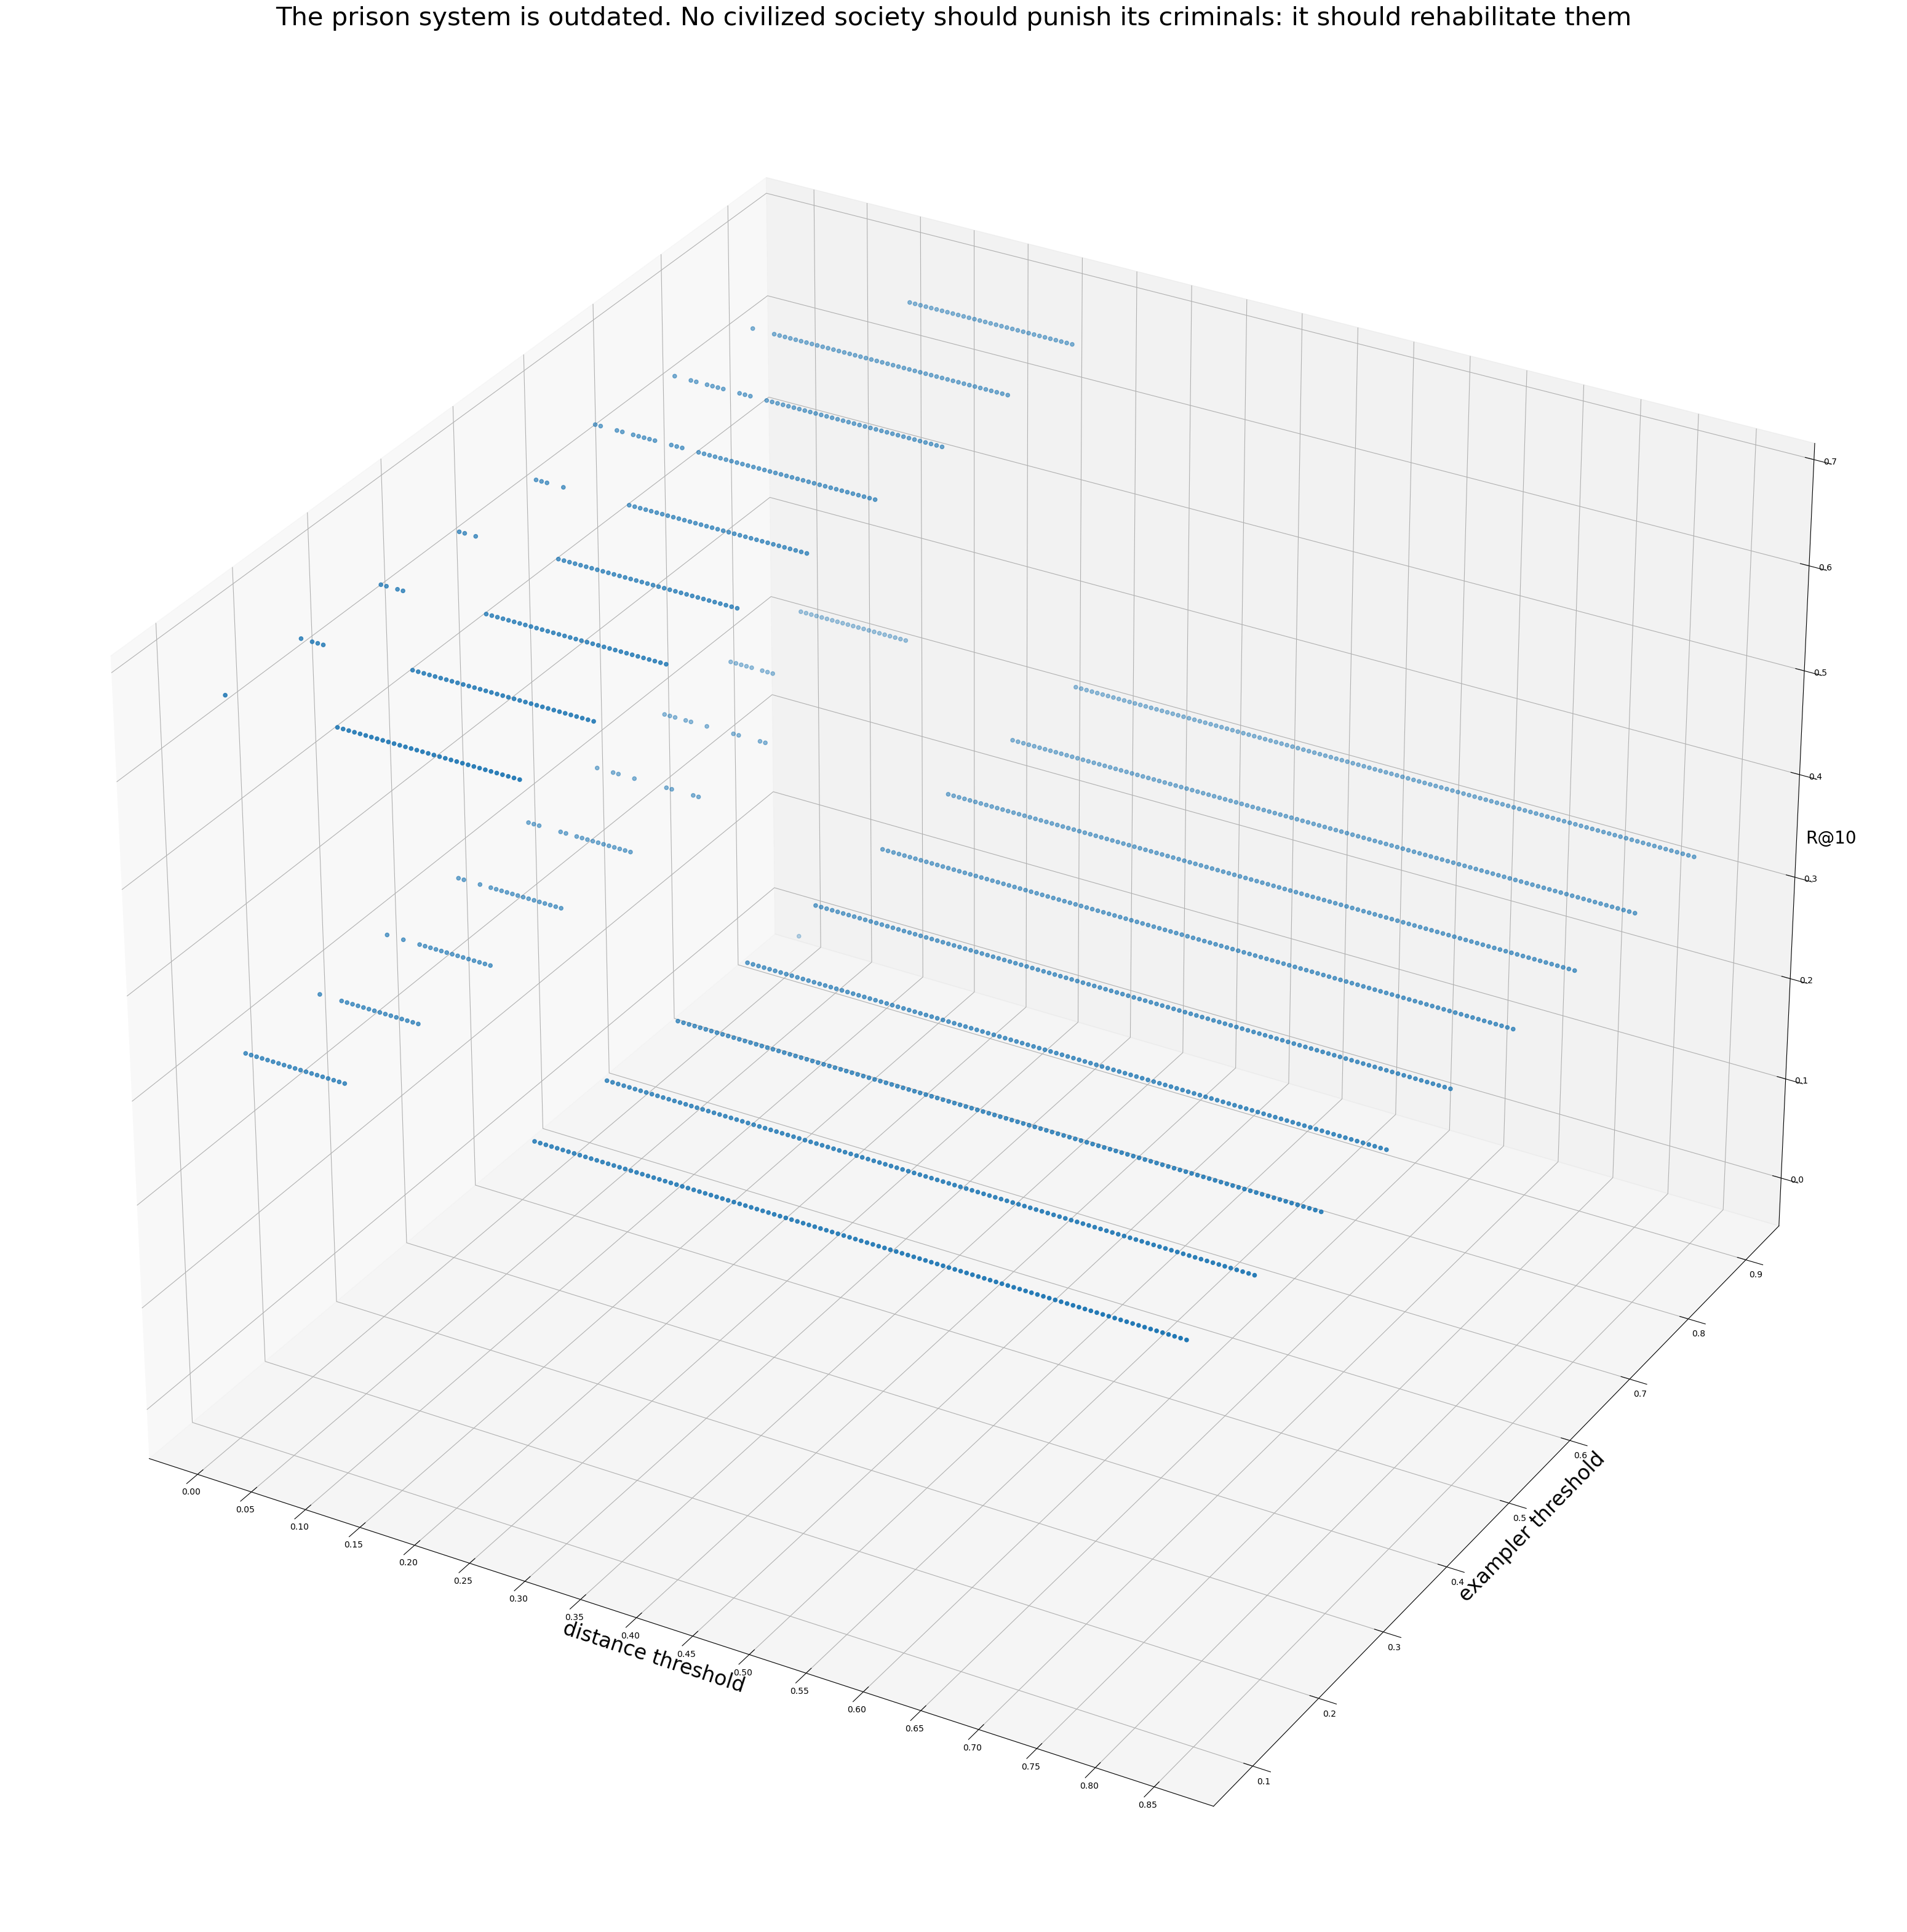
\includegraphics[width=1.0\linewidth]{prompt_0005_R@10.png}
  \caption{distance\_threshold、example\_threshold、R@10变化趋势(BERT分类模型[CLS])}
  \label{framework}
\end{figure*}

\begin{figure*}[htbp]\small
  \centering
  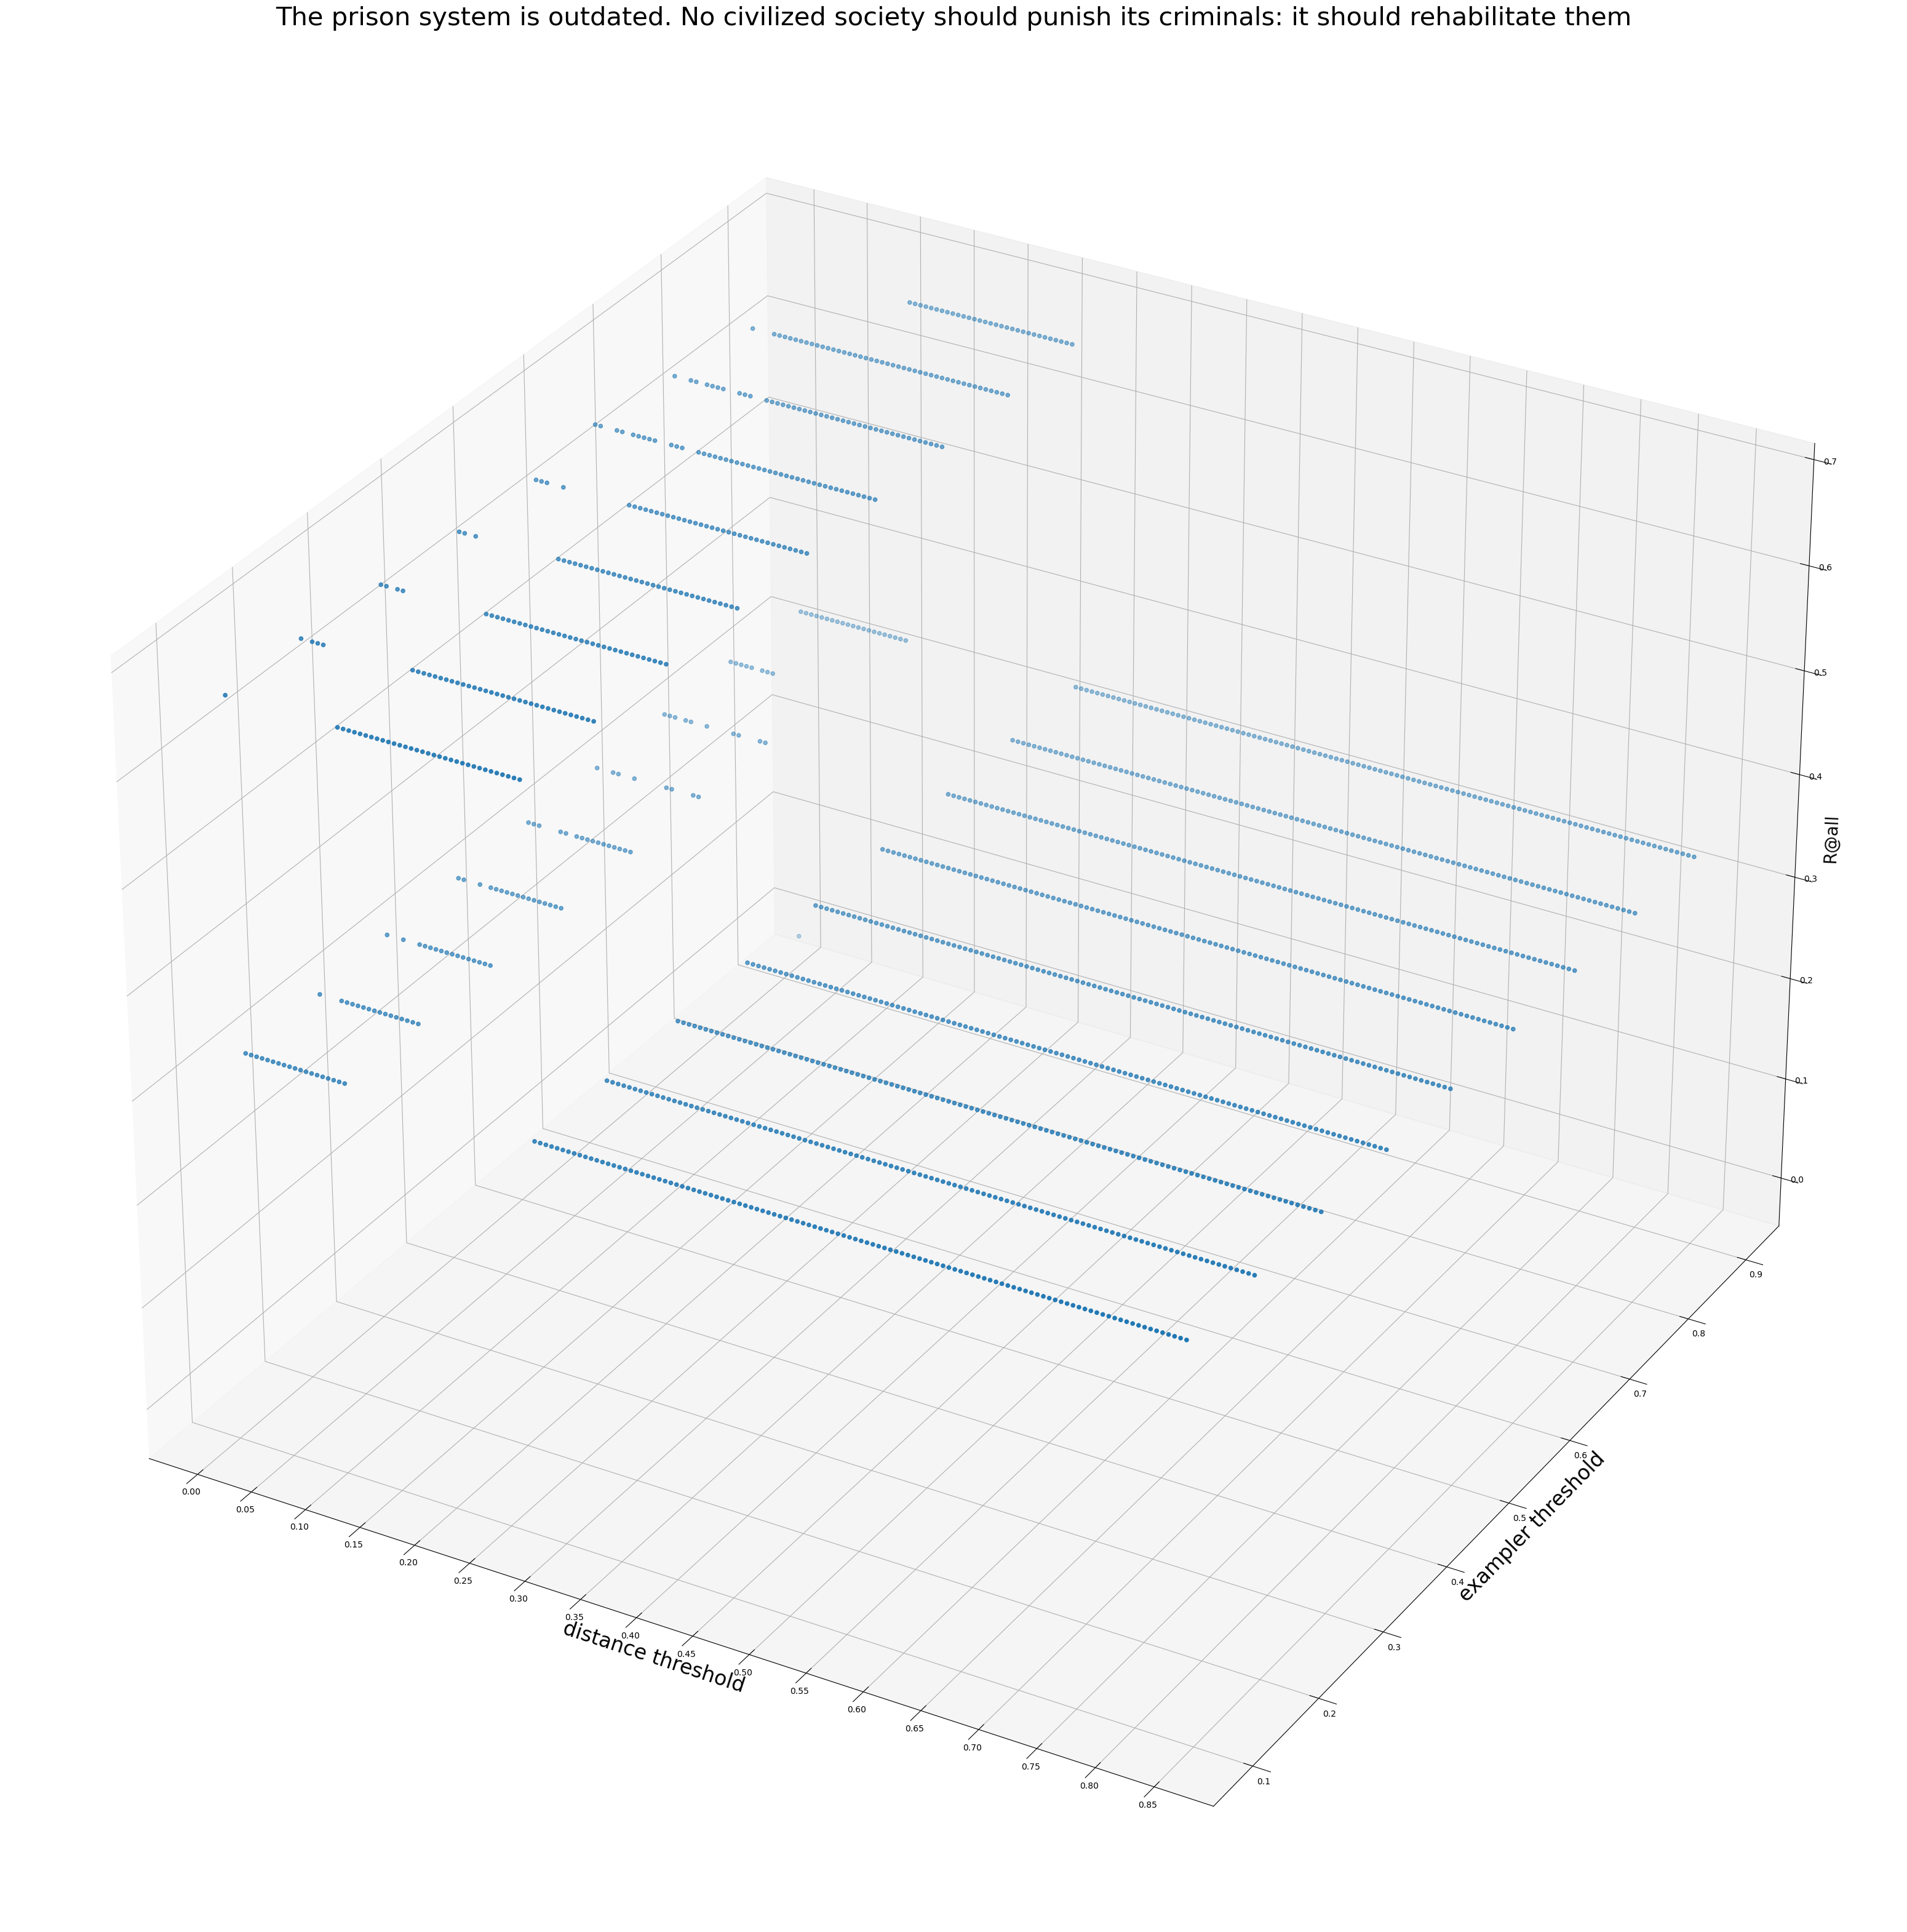
\includegraphics[width=1.0\linewidth]{prompt_0005_R@all.png}
  \caption{distance\_threshold、example\_threshold、R@all变化趋势(BERT分类模型[CLS])}
  \label{framework}
\end{figure*}

\subsection{方案一算法}

\begin{algorithm}[htbp]
    \caption{Clustering-based Essay Topical Relevance Assessment}
    \label{}
    \begin{algorithmic}[1]
        \REQUIRE ~~\\ %算法的输入参数:Input
            $V:$ A list of feature vectors for essays from a given prompt; \\
            $T:$ Similarity threshold for agglomerative clustering; \\
            \textbf{ExemplarChecker}: A function to check whether an essay cluster could be viewed as a topic exemplar.
        \ENSURE ~~\\ %算法的输出:Output
            $R:$ Essays ranked according to the probability of being off-topic. \\ 
        \STATE Applying AgglomerativeClustering algorithm to cluster $V$ into clusters $\left\{C_{1}, \ldots, C_{m}\right\}$ with the Similarity constraint $T$. \
        \STATE $E=[]$ // Topic Exxemplars \
        \STATE $O=[]$ // Outliers \
        \FOR{each cluster $C_{i}$}
            \IF{ExemplarChecker($C_i$) is True}
                \STATE $E$.append($C_{i}$)\
            \ELSE
                \STATE $O$.append($C_{i}$)\
            \ENDIF
        \ENDFOR
        \STATE $S=[]$ // Scores \
        \FOR{$x$ in $O$}
            \STATE $score(x)=max_{C_i \in E}(Sim([x], C_i))$ \
            \STATE $S$.append($score(x)$) \
        \ENDFOR

        \STATE R = Ranking(O, S) // Rank $O$ according to $S$ in ascending order \
        \STATE \textbf{return} R\
    \end{algorithmic}
\end{algorithm}

\subsection{中文35个主题指标}

% Table generated by Excel2LaTeX from sheet '中文'
\begin{table}[hp]
  \centering
  \resizebox*{\textwidth}{!}{
    \begin{tabular}{c|c|ccccccccc}
      \hline
      \multicolumn{2}{c|}{} & \textbf{R@10} & \textbf{R@15} & \textbf{R@20} & \textbf{R@50} & \textbf{R@all} & \textbf{P@1} & \textbf{P@5} & \textbf{P@10} & \textbf{spearman} \\
      \hline
      \multicolumn{2}{c|}{\textbf{tfidf}} &       &       &       &       &       &       &       &       &  \\
      \hline
      \multicolumn{2}{c|}{\textbf{doc2vec}} & 0.0593  & 0.0761  & 0.0977  & 0.1971  & -     & 0.4000  & 0.2743  & 0.2343  & 0.1102  \\
      \hline
      \multirow{10}[0]{*}{\textbf{分类模型}} & \textbf{lstm} & 0.0531  & 0.0719  & 0.0816  & 0.1708  & -     & 0.2286  & 0.2400  & 0.2171  & 0.1133  \\
      & \textbf{lstm(+测试主题)} & \textcolor[rgb]{ 1,  0,  0}{\textbf{0.0664 }} & 0.0903  & 0.1091  & 0.1976  & -     & 0.4286  & 0.3143  & 0.2714  & 0.1273  \\
      \cline{2-11}
      & \textbf{bert\_CLS} & 0.0491  & 0.0643  & 0.0779  & 0.1473  & -     & 0.3714  & 0.2400  & 0.1943  & 0.0920  \\
      & \textbf{bert\_CLS(+whitening)} & 0.0231  & 0.0315  & 0.0394  & 0.1061  & -     & 0.0571  & 0.0857  & 0.0914  & 0.0869  \\
      & \textbf{bert\_CLS(+测试主题)} & 0.0570  & 0.0741  & 0.0940  & 0.1685  & -     & 0.2286  & 0.2457  & 0.2257  & 0.1059  \\
      & \textbf{bert\_CLS(+测试主题,+whitening)} & 0.0264  & 0.0367  & 0.0468  & 0.1103  & -     & 0.0857  & 0.1029  & 0.1057  & 0.0966  \\
      \cline{2-11}
      & \textbf{bert\_Last1avg} & 0.0531  & 0.0704  & 0.0855  & 0.1629  & -     & 0.3143  & 0.2514  & 0.2057  & 0.0880  \\
      & \textbf{bert\_Last1avg(+whitening)} & 0.0252  & 0.0371  & 0.0509  & 0.1187  & -     & 0.1143  & 0.1143  & 0.0971  & 0.0940  \\
      & \textbf{bert\_Last1avg(+测试主题)} & 0.0622  & 0.0908  & 0.1105  & 0.1963  & -     & 0.4571  & 0.2914  & 0.2400  & 0.1188  \\
      & \textbf{bert\_Last1avg(+测试主题,+whitening)} & 0.0284  & 0.0419  & 0.0614  & 0.1436  & -     & 0.1143  & 0.1086  & 0.1114  & 0.1136  \\
      \hline
      \multirow{10}[0]{*}{\textbf{生成模型}} & \textbf{lstm\_$\rm h_{t_n}$} & 0.0081  & 0.0126  & 0.0162  & 0.0479  & -     & 0.0000  & 0.0457  & 0.0343  & 0.0123  \\
      & \textbf{lstm\_avg} & 0.0442  & 0.0607  & 0.0734  & 0.1408  & -     & 0.2000  & 0.2057  & 0.1743  & 0.0810  \\
      \cline{2-11}
      & \textbf{bert\_CLS} & 0.0560  & 0.0736  & 0.0860  & 0.1426  & -     & 0.3143  & 0.2686  & 0.2257  & 0.0666  \\
      & \textbf{bert\_CLS(+whitening)} & 0.0364  & 0.0472  & 0.0605  & 0.1185  & -     & 0.0571  & 0.1371  & 0.1429  & 0.0858  \\
      & \textbf{bert\_CLS(+测试作文)} & 0.0312  & 0.0414  & 0.0522  & 0.1064  & -     & 0.2286  & 0.1600  & 0.1314  & 0.0410  \\
      & \textbf{bert\_CLS(+测试作文,+wihtening)} & 0.0289  & 0.0415  & 0.0514  & 0.1172  & -     & 0.0857  & 0.1143  & 0.1143  & 0.0757  \\
      \cline{2-11}
      & \textbf{bert\_Last1avg} & 0.0350  & 0.0433  & 0.0535  & 0.1061  & -     & 0.1714  & 0.1429  & 0.1371  & 0.0581  \\
      & \textbf{bert\_Last1avg(+whitening)} & 0.0271  & 0.0379  & 0.0492  & 0.1140  & -     & 0.0857  & 0.1086  & 0.1114  & 0.0846  \\
      & \textbf{bert\_Last1avg(+测试作文)} & 0.0401  & 0.0510  & 0.0596  & 0.1129  & -     & 0.3714  & 0.1943  & 0.1686  & 0.0438  \\
      & \textbf{bert\_Last1avg(+测试作文,+whitening)} & 0.0292  & 0.0422  & 0.0512  & 0.1080  & -     & 0.0571  & 0.1600  & 0.1114  & 0.0697  \\
      \hline
    \end{tabular}}%
    \begin{tablenotes}    %这行要添加, 从这开始
      \footnotesize               %这行要添加
      \item[1] R@all 表示全部小类中离题的召回
      \item[2] +测试主题 表示在测试主题继续训练分类模型
      \item[3] +测试作文 表示在测试集上继续训练生成模型
      \item[4] +whitening 表示使用Bert-whitening对表示进行变换
      \item[5] * lstm\_$\rm h_{t_n}$ 表示取Lstm最后时刻的表示,lstm\_avg 表示取Lstm所有时刻的表示平均 
    \end{tablenotes} 
    \caption{聚类方案二(one-class)指标更新(中文-35主题)}
  \label{tab:addlabel}%
\end{table}%

% Table generated by Excel2LaTeX from sheet '中文'
\begin{table}[htbp]
  \centering
  \resizebox*{\textwidth}{!}{
    \begin{tabular}{c|c|ccccccccc}
      \hline
      \multicolumn{2}{c|}{} & \textbf{R@10} & \textbf{R@15} & \textbf{R@20} & \textbf{R@50} & \textbf{R@all} & \textbf{P@1} & \textbf{P@5} & \textbf{P@10} & \textbf{spearman} \\
      \hline
      \multicolumn{2}{c|}{\textbf{tfidf}} &       &       &       &       &       &       &       &       &  \\
      \hline
      \multicolumn{2}{c|}{\textbf{doc2vec}} & 0.0356  & 0.0480  & 0.0635  & 0.1269  & -     & 0.2857  & 0.1429  & 0.1400  & 0.0440  \\
      \hline
      \multirow{10}[0]{*}{\textbf{分类模型}} & \textbf{lstm} & 0.0104  & 0.0182  & 0.0219  & 0.0468  & -     & 0.0857  & 0.0457  & 0.0371  & -0.0172  \\
      & \textbf{lstm(+测试主题)} & 0.0086  & 0.0114  & 0.0207  & 0.0616  & -     & 0.0286  & 0.0286  & 0.0343  & -0.0190  \\
      \cline{2-11}
      & \textbf{bert\_CLS} & 0.0219  & 0.0345  & 0.0463  & 0.1078  & -     & 0.2000  & 0.1086  & 0.0886  & 0.0789  \\
      & \textbf{bert\_CLS(+whitening)} & 0.0100  & 0.0195  & 0.0249  & 0.0715  & -     & 0.0000  & 0.0286  & 0.0371  & 0.0416  \\
      & \textbf{bert\_CLS(+测试主题)} & 0.0453  & 0.0642  & 0.0775  & 0.1580  & -     & 0.2000  & 0.2171  & 0.1829  & 0.0996  \\
      & \textbf{bert\_CLS(+测试主题,+whitening)} & 0.0122  & 0.0152  & 0.0237  & 0.0634  & -     & 0.0000  & 0.0286  & 0.0457  & 0.0521  \\
      \cline{2-11}
      & \textbf{bert\_Last1avg} & 0.0417  & 0.0543  & 0.0723  & 0.1522  & -     & 0.3143  & 0.2171  & 0.1686  & 0.0919  \\
      & \textbf{bert\_Last1avg(+whitening)} & 0.0101  & 0.0142  & 0.0198  & 0.0504  & -     & 0.0286  & 0.0343  & 0.0400  & 0.0267  \\
      & \textbf{bert\_Last1avg(+测试主题)} & 0.0582  & 0.0741  & 0.0881  & 0.1739  & -     & 0.3143  & 0.2229  & 0.2286  & 0.1091  \\
      & \textbf{bert\_Last1avg(+测试主题,+whitening)} & 0.0123  & 0.0202  & 0.0289  & 0.0765  & -     & 0.0857  & 0.0457  & 0.0486  & 0.0544  \\
      \hline
      \multirow{10}[0]{*}{\textbf{生成模型}} & \textbf{lstm\_$\rm h_{t_n}$} & 0.0155  & 0.0237  & 0.0334  & 0.0669  & -     & 0.0571  & 0.0571  & 0.0629  & 0.0259  \\
      & \textbf{lstm\_avg} & 0.0236  & 0.0309  & 0.0363  & 0.0649  & -     & 0.1714  & 0.0857  & 0.0943  & -0.0215  \\
      \cline{2-11}
      & \textbf{bert\_CLS} & 0.0580  & 0.0765  & 0.0874  & 0.1544  & -     & 0.3429  & 0.2800  & 0.2429  & 0.0813  \\
      & \textbf{bert\_CLS(+whitening)} & 0.0121  & 0.0146  & 0.0174  & 0.0480  & -     & 0.0000  & 0.0400  & 0.0457  & 0.0081  \\
      & \textbf{bert\_CLS(+测试作文)} & 0.0303  & 0.0428  & 0.0548  & 0.1030  & -     & 0.2000  & 0.1371  & 0.1286  & 0.0338  \\
      & \textbf{bert\_CLS(+测试作文,+wihtening)} & 0.0099  & 0.0142  & 0.0175  & 0.0503  & -     & 0.0571  & 0.0286  & 0.0371  & 0.0106  \\
      \cline{2-11}
      & \textbf{bert\_Last1avg} & 0.0313  & 0.0411  & 0.0507  & 0.1003  & -     & 0.1143  & 0.1600  & 0.1371  & 0.0489  \\
      & \textbf{bert\_Last1avg(+whitening)} & 0.0076  & 0.0119  & 0.0171  & 0.0460  & -     & 0.0286  & 0.0286  & 0.0286  & 0.0012  \\
      & \textbf{bert\_Last1avg(+测试作文)} & 0.0400  & 0.0486  & 0.0607  & 0.1139  & -     & 0.3714  & 0.1771  & 0.1657  & 0.0237  \\
      & \textbf{bert\_Last1avg(+测试作文,+whitening)} & 0.0131  & 0.0170  & 0.0214  & 0.0534  & -     & 0.0571  & 0.0400  & 0.0457  & 0.0097  \\
      \hline
    \end{tabular}}%
    \begin{tablenotes}    %这行要添加, 从这开始
      \footnotesize               %这行要添加
      \item[1] R@all 表示全部小类中离题的召回
      \item[2] +作文 表示在作文数据上进行微调(原始模型使用新闻数据预训练) 
      \item[3] +whitening 表示使用Bert-whitening对表示进行变换
      \item[4] * lstm\_$\rm h_{t_n}$ 表示取Lstm最后时刻的表示,lstm\_avg 表示取Lstm所有时刻的表示平均
    \end{tablenotes} 
    \caption{聚类方案四指标更新(中文-35主题)}
  \label{tab:addlabel}%
\end{table}%

\end{CJK}
\end{document}

% include your own bib file like this:


%\begin{thebibliography}{}

%\bibitem[\protect\citename{Aho and Ullman}1972]{Aho:72}
%Alfred~V. Aho and Jeffrey~D. Ullman.
%\newblock 1972.
%\newblock {\em The Theory of Parsing, Translation and Compiling}, volume~1.
%\newblock Prentice-{Hall}, Englewood Cliffs, NJ.

%\bibitem[\protect\citename{{American Psychological Association}}1983]{APA:83}
%{American Psychological Association}.
%\newblock 1983.
%\newblock {\em Publications Manual}.
%\newblock American Psychological Association, Washington, DC.

%\bibitem[\protect\citename{{Association for Computing Machinery}}1983]{ACM:83}
%{Association for Computing Machinery}.
%\newblock 1983.
%\newblock {\em Computing Reviews}, 24(11):503--512.

%\bibitem[\protect\citename{Chandra \bgroup et al.\egroup }1981]{Chandra:81}
%Ashok~K. Chandra, Dexter~C. Kozen, and Larry~J. Stockmeyer.
%\newblock 1981.
%\newblock Alternation.
%\newblock {\em Journal of the Association for Computing Machinery},
%  28(1):114--133.

%\bibitem[\protect\citename{Gusfield}1997]{Gusfield:97}
%Dan Gusfield.
%\newblock 1997.
%\newblock {\em Algorithms on Strings, Trees and Sequences}.
%\newblock Cambridge University Press, Cambridge, UK.

%\bibitem[\protect\citename{Rasooli and Tetreault}2015]{rasooli-tetrault-2015}
%Mohammad~Sadegh Rasooli and Joel~R. Tetreault. 2015.
%\newblock {Yara parser: {A} fast and accurate dependency parser}.
%\newblock \emph{Computing Research Repository}, arXiv:1503.06733.
%\newblock Version 2.

%\bibitem[\protect\citename{Borschinger and Johnson}2011]{borsch2011}
%Benjamin Borschinger and Mark Johnson. 2011.
%\newblock A particle filter algorithm for {B}ayesian wordsegmentation.
%\newblock In \emph{Proceedings of the Australasian Language Technology Association %Workshop 2011}, pages 10--18, Canberra, Australia.

%\end{thebibliography}

